% Options for packages loaded elsewhere
\PassOptionsToPackage{unicode}{hyperref}
\PassOptionsToPackage{hyphens}{url}
%
\documentclass[
  man]{apa6}
\usepackage{amsmath,amssymb}
\usepackage{iftex}
\ifPDFTeX
  \usepackage[T1]{fontenc}
  \usepackage[utf8]{inputenc}
  \usepackage{textcomp} % provide euro and other symbols
\else % if luatex or xetex
  \usepackage{unicode-math} % this also loads fontspec
  \defaultfontfeatures{Scale=MatchLowercase}
  \defaultfontfeatures[\rmfamily]{Ligatures=TeX,Scale=1}
\fi
\usepackage{lmodern}
\ifPDFTeX\else
  % xetex/luatex font selection
\fi
% Use upquote if available, for straight quotes in verbatim environments
\IfFileExists{upquote.sty}{\usepackage{upquote}}{}
\IfFileExists{microtype.sty}{% use microtype if available
  \usepackage[]{microtype}
  \UseMicrotypeSet[protrusion]{basicmath} % disable protrusion for tt fonts
}{}
\makeatletter
\@ifundefined{KOMAClassName}{% if non-KOMA class
  \IfFileExists{parskip.sty}{%
    \usepackage{parskip}
  }{% else
    \setlength{\parindent}{0pt}
    \setlength{\parskip}{6pt plus 2pt minus 1pt}}
}{% if KOMA class
  \KOMAoptions{parskip=half}}
\makeatother
\usepackage{xcolor}
\usepackage{graphicx}
\makeatletter
\def\maxwidth{\ifdim\Gin@nat@width>\linewidth\linewidth\else\Gin@nat@width\fi}
\def\maxheight{\ifdim\Gin@nat@height>\textheight\textheight\else\Gin@nat@height\fi}
\makeatother
% Scale images if necessary, so that they will not overflow the page
% margins by default, and it is still possible to overwrite the defaults
% using explicit options in \includegraphics[width, height, ...]{}
\setkeys{Gin}{width=\maxwidth,height=\maxheight,keepaspectratio}
% Set default figure placement to htbp
\makeatletter
\def\fps@figure{htbp}
\makeatother
\setlength{\emergencystretch}{3em} % prevent overfull lines
\providecommand{\tightlist}{%
  \setlength{\itemsep}{0pt}\setlength{\parskip}{0pt}}
\setcounter{secnumdepth}{-\maxdimen} % remove section numbering
% Make \paragraph and \subparagraph free-standing
\makeatletter
\ifx\paragraph\undefined\else
  \let\oldparagraph\paragraph
  \renewcommand{\paragraph}{
    \@ifstar
      \xxxParagraphStar
      \xxxParagraphNoStar
  }
  \newcommand{\xxxParagraphStar}[1]{\oldparagraph*{#1}\mbox{}}
  \newcommand{\xxxParagraphNoStar}[1]{\oldparagraph{#1}\mbox{}}
\fi
\ifx\subparagraph\undefined\else
  \let\oldsubparagraph\subparagraph
  \renewcommand{\subparagraph}{
    \@ifstar
      \xxxSubParagraphStar
      \xxxSubParagraphNoStar
  }
  \newcommand{\xxxSubParagraphStar}[1]{\oldsubparagraph*{#1}\mbox{}}
  \newcommand{\xxxSubParagraphNoStar}[1]{\oldsubparagraph{#1}\mbox{}}
\fi
\makeatother
% definitions for citeproc citations
\NewDocumentCommand\citeproctext{}{}
\NewDocumentCommand\citeproc{mm}{%
  \begingroup\def\citeproctext{#2}\cite{#1}\endgroup}
\makeatletter
 % allow citations to break across lines
 \let\@cite@ofmt\@firstofone
 % avoid brackets around text for \cite:
 \def\@biblabel#1{}
 \def\@cite#1#2{{#1\if@tempswa , #2\fi}}
\makeatother
\newlength{\cslhangindent}
\setlength{\cslhangindent}{1.5em}
\newlength{\csllabelwidth}
\setlength{\csllabelwidth}{3em}
\newenvironment{CSLReferences}[2] % #1 hanging-indent, #2 entry-spacing
 {\begin{list}{}{%
  \setlength{\itemindent}{0pt}
  \setlength{\leftmargin}{0pt}
  \setlength{\parsep}{0pt}
  % turn on hanging indent if param 1 is 1
  \ifodd #1
   \setlength{\leftmargin}{\cslhangindent}
   \setlength{\itemindent}{-1\cslhangindent}
  \fi
  % set entry spacing
  \setlength{\itemsep}{#2\baselineskip}}}
 {\end{list}}
\usepackage{calc}
\newcommand{\CSLBlock}[1]{\hfill\break\parbox[t]{\linewidth}{\strut\ignorespaces#1\strut}}
\newcommand{\CSLLeftMargin}[1]{\parbox[t]{\csllabelwidth}{\strut#1\strut}}
\newcommand{\CSLRightInline}[1]{\parbox[t]{\linewidth - \csllabelwidth}{\strut#1\strut}}
\newcommand{\CSLIndent}[1]{\hspace{\cslhangindent}#1}
\ifLuaTeX
\usepackage[bidi=basic]{babel}
\else
\usepackage[bidi=default]{babel}
\fi
\babelprovide[main,import]{english}
% get rid of language-specific shorthands (see #6817):
\let\LanguageShortHands\languageshorthands
\def\languageshorthands#1{}
% Manuscript styling
\usepackage{upgreek}
\captionsetup{font=singlespacing,justification=justified}

% Table formatting
\usepackage{longtable}
\usepackage{lscape}
% \usepackage[counterclockwise]{rotating}   % Landscape page setup for large tables
\usepackage{multirow}		% Table styling
\usepackage{tabularx}		% Control Column width
\usepackage[flushleft]{threeparttable}	% Allows for three part tables with a specified notes section
\usepackage{threeparttablex}            % Lets threeparttable work with longtable

% Create new environments so endfloat can handle them
% \newenvironment{ltable}
%   {\begin{landscape}\centering\begin{threeparttable}}
%   {\end{threeparttable}\end{landscape}}
\newenvironment{lltable}{\begin{landscape}\centering\begin{ThreePartTable}}{\end{ThreePartTable}\end{landscape}}

% Enables adjusting longtable caption width to table width
% Solution found at http://golatex.de/longtable-mit-caption-so-breit-wie-die-tabelle-t15767.html
\makeatletter
\newcommand\LastLTentrywidth{1em}
\newlength\longtablewidth
\setlength{\longtablewidth}{1in}
\newcommand{\getlongtablewidth}{\begingroup \ifcsname LT@\roman{LT@tables}\endcsname \global\longtablewidth=0pt \renewcommand{\LT@entry}[2]{\global\advance\longtablewidth by ##2\relax\gdef\LastLTentrywidth{##2}}\@nameuse{LT@\roman{LT@tables}} \fi \endgroup}

% \setlength{\parindent}{0.5in}
% \setlength{\parskip}{0pt plus 0pt minus 0pt}

% Overwrite redefinition of paragraph and subparagraph by the default LaTeX template
% See https://github.com/crsh/papaja/issues/292
\makeatletter
\renewcommand{\paragraph}{\@startsection{paragraph}{4}{\parindent}%
  {0\baselineskip \@plus 0.2ex \@minus 0.2ex}%
  {-1em}%
  {\normalfont\normalsize\bfseries\itshape\typesectitle}}

\renewcommand{\subparagraph}[1]{\@startsection{subparagraph}{5}{1em}%
  {0\baselineskip \@plus 0.2ex \@minus 0.2ex}%
  {-\z@\relax}%
  {\normalfont\normalsize\itshape\hspace{\parindent}{#1}\textit{\addperi}}{\relax}}
\makeatother

\makeatletter
\usepackage{etoolbox}
\patchcmd{\maketitle}
  {\section{\normalfont\normalsize\abstractname}}
  {\section*{\normalfont\normalsize\abstractname}}
  {}{\typeout{Failed to patch abstract.}}
\patchcmd{\maketitle}
  {\section{\protect\normalfont{\@title}}}
  {\section*{\protect\normalfont{\@title}}}
  {}{\typeout{Failed to patch title.}}
\makeatother

\usepackage{xpatch}
\makeatletter
\xapptocmd\appendix
  {\xapptocmd\section
    {\addcontentsline{toc}{section}{\appendixname\ifoneappendix\else~\theappendix\fi\\: #1}}
    {}{\InnerPatchFailed}%
  }
{}{\PatchFailed}
\keywords{Latent interaction, UPI, RAPI, 2S-PA}
\DeclareDelayedFloatFlavor{ThreePartTable}{table}
\DeclareDelayedFloatFlavor{lltable}{table}
\DeclareDelayedFloatFlavor*{longtable}{table}
\makeatletter
\renewcommand{\efloat@iwrite}[1]{\immediate\expandafter\protected@write\csname efloat@post#1\endcsname{}}
\makeatother
\usepackage{lineno}

\linenumbers
\usepackage{csquotes}
\ifLuaTeX
  \usepackage{selnolig}  % disable illegal ligatures
\fi
\usepackage{bookmark}
\IfFileExists{xurl.sty}{\usepackage{xurl}}{} % add URL line breaks if available
\urlstyle{same}
\hypersetup{
  pdftitle={Two-Stage Path Analysis with Interaction: A Good Alternative to Current Methods of Modeling Latent Interaction},
  pdfauthor={Gengrui (Jimmy) Zhang1},
  pdflang={en-EN},
  pdfkeywords={Latent interaction, UPI, RAPI, 2S-PA},
  hidelinks,
  pdfcreator={LaTeX via pandoc}}

\title{Two-Stage Path Analysis with Interaction: A Good Alternative to Current Methods of Modeling Latent Interaction}
\author{Gengrui (Jimmy) Zhang\textsuperscript{1}}
\date{}


\shorttitle{2S-PA-Int}

\authornote{

The authors made the following contributions. Gengrui (Jimmy) Zhang: Conceptualization, Writing - Original Draft Preparation, Writing - Review \& Editing.

Correspondence concerning this article should be addressed to Gengrui (Jimmy) Zhang. E-mail: \href{mailto:gengruiz@email.com}{\nolinkurl{gengruiz@email.com}}

}

\affiliation{\vspace{0.5cm}\textsuperscript{1} University of Southhern California}

\abstract{%
Modeling interaction effects within the latent variable modeling framework has become increasingly popular in psychological research as it facilitates the exploration of in-depth theory and complex data structure. Comprared to the extensitvely used regression-based approaches assuming error-free variables, the latent interaction approach is able to account for measurement error and produce estimates with less bias and more accurate standard error. In this study, we investigated three product indicator methods based on structural equation modeling (SEM): Matched-pair Unconstrained Product Indicator (UPI), Reliability-Adjusted Product Indicator (RAPI), and an extended model based on the two-stage path analysis (2S-PA) framework, namely 2S-PA-Int, by conducting a simulation study with 2,000 replications. The results showed that 2S-PA-Int produced consistently less standardized bias, acceptable relative SE bias and coverage rates, and lower RMSE values than matched-pair UPI and RAPI, particularly under the conditions of small sample size and low reliability. Generally, 2S-PA-Int showed promising statistical properties and simpler model specification, indicating that it could serve as a competitive alternative of existing methods. Future research directions of 2S-PA-Int were discussed.
}



\begin{document}
\maketitle

Social science research increasingly focuses on intricate dynamics of complex phenomena, such as nonlinear and moderation effects, rather than merely simple bivariate relationship. This shift reflects the multifaceted nature of the real world, which seldom conforms to straightforward patterns (Carte \& Russell, 2003; Cunningham \& Ahn, 2019; MacKinnon \& Luecken, 2008). For instance, while earlier studies have established that exercise contributes to weight loss, there is a burgeoning interest in understanding and probing into the underlying mechanisms, such as optimal timing, specific target populations, and the contextual conditions that modulate the effectiveness of exercise in promoting weight loss. Investigations into moderation, or interaction effects, provide critical insights into these inquiries by examining how additional variables---or an ensemble of variables---shape the dynamics between the primary variables of interest.

A prevalent approach to modeling moderation is through regression analysis, specifically by incorporating an interaction term, \(XZ\):
\begin{equation}
Y = b_{0} + b_{1}X + b_{2}Z + b_{3}XZ + \epsilon,
\end{equation}
where \(b_{0}\) is the intercept, \(b_{1}\) and \(b_{2}\) are the regression coefficients for \(X\) and \(Z\) respectively, \(b_{3}\) is the coefficient for the interaction term \(XZ\), and \(\epsilon\) is the error term. To maintain consistency with the naming convention used by Marsh et al. (2004), we refer to main effects (i.e., non-interaction effects) as ``first-order effects''. Hence \(X\) and \(Z\) are first-order variables and \(b_{1}\) and \(b_{2}\) are first-order effects in this case.

Classical regression model typically assumes that variables are measured without error, a premise that can lead to biased parameter estimates when measurement errors are present in empirical research (Bollen, 1989; Carroll et al., 2006; Cohen et al., 2003). This bias may be particularly more inflated for interaction effects (Anderson et al., 1996). To mitigate this issue, researchers use latent variables that are inferred and measured by a set of observed indicators within the structural equation modeling (SEM) framework, which can control and accommodate measurement errors in observed indicators (Bollen, 2002). For example, depression is widely measured and assessed using the Center for Epidemiologic Studies Depression (CES-D) scale consisting of 20 items (Radloff, 1977). An expanding body of research has demonstrated that SEM-based moderation models reliably provide more accurate representations of the relationships among latent constructs (Cham et al., 2012; Maslowsky et al., 2015; Mueller, 1997; Steinmetz et al., 2011).

The Two-Stage Path Analysis (2S-PA; Lai \& Hsiao, 2022) method models pathway relationships among latent variables through the use of factor scores. Simulation studies have shown its ability to yield parameter estimates with reduced standard error bias, enhanced convergence rates, and improved management of Type I error, particularly in small sample contexts (Lai et al., 2023; Lai \& Hsiao, 2022). Given its promising statistical property, simpler model specification, and easier implementation in widely used software, we extended the 2S-PA method to incorporate latent interaction estimation in this study, and named it 2S-PA-Int. We reviewed two widely used latent interaction models using the product indicator method: Unconstrained Product Indicator with Matched Pairs (Matched-Pair UPI; Marsh et al., 2004) and Reliability-Adjusted Product Indicator (RAPI; Hsiao et al., 2018). Then we conducted a Monte Carlo simulation study to compare their performance with 2S-PA-Int. To proceed, we first introduced a classical model of latent interaction, and then presented UPI, RAPI, and 2S-PA-Int with technical details.

\subsection{A Classical Model of Latent Interaction}\label{a-classical-model-of-latent-interaction}

Kenny and Judd (1984) introduced a seminal structural model for estimating latent interaction effects, particularly in scenarios involving two latent predictors and their interaction term:
\begin{equation}
y = \alpha + \gamma_{x}\xi_{x} + \gamma_{m}\xi_{m} + \gamma_{xm}\xi_{x}\xi_{m} + \zeta,
\end{equation}
where \(\alpha\) is the constant intercept, \(\xi_{x}\) and \(\xi_{m}\) are the first-order latent predictors, and the product \(\xi_{x}\xi_{m}\) defines the interaction effect. Note that \(\xi_{x}\) and \(\xi_{m}\) are allowed to correlate with each other. The disturbance term \(\zeta\) in the model is assumed to follow a normal distribution, \(\zeta \sim N(0, \psi)\), where \(\psi\) denotes the variance of \(\zeta\), accounting for unobserved factors that influence the dependent variable. The coefficients \(\gamma_{x}\) and \(\gamma_{m}\) capture the first-order effects of the latent predictors, while \(\gamma_{xm}\) measures the latent interaction effect. The dependent variable \(y\) in this model can be either an observed variable or a latent construct, allowing for flexibility in its application.

The measurement model for the first-order latent predictors, such as \(\xi_{x}\), can be articulated by the following confirmatory factor analysis (CFA) framework:
\begin{equation}
\mathbf{x} = \boldsymbol{\tau_{x}} + \boldsymbol{\lambda_{x}}\xi_{x} + \boldsymbol{\delta_{x}},
\end{equation}
wherein, for each indicator \(i = 1, \ 2, \ ..., \ p\) associated with the latent predictor \(\xi_{x}\), \(\mathbf{x}\) denotes a \(p \times 1\) vector of observed first-order indicators (i.e., the indicators of \(\xi_{x}\)). The term \(\boldsymbol{\tau_{x}}\) represents a \(p \times 1\) vector of constant intercepts, while \(\boldsymbol{\lambda}{x}\) is a \(p \times 1\) vector of factor loadings, which capture the strength of the relationship between the latent variable \(\xi{x}\) and each of its indicators. The vector \(\boldsymbol{\delta_{x}}\) represents the \(p \times 1\) vector of measurement errors associated with these indicators. Each measurement error \(\delta_{x_{i}}\) is normally distributed with a mean of zero and a variance of \(\theta_{x_{i}}\). Under the assumption of local independence, which posits that the first-order indicators are uncorrelated with one another when they are indicators of the same latent variable, the variance-covariance matrix of all the indicators' measurement errors is a diagonal matrix, denoted as \(\mathbf{\Theta_{\delta_{x}}} = \text{diag}(\theta_{x_{1}}, \theta_{x_{2}}, ..., \theta_{x_{p}})\). This measurement model, along with its associated parameters, is similarly applicable to the latent predictor \(\xi_{m}\), ensuring consistency in the modeling of both latent variables.

Kenny and Judd's original formulation of model omitted the intercept \(\alpha\), a point subsequently addressed by Jöreskog and Yang (1996), who revised the model under a set of assumptions. The revised latent interaction model is grounded in three primary assumptions related to multivariate normal distribution and independence: (1) The measurement errors of first-order indicators, the first-order latent predictors, and the disturbance term in the structural model are multivariate normal, uncorrelated, and independent to each other (i.e., \(Corr[\delta, \xi] = 0\); \(Corr[\zeta, \xi] = 0\); \(Corr[\delta, \zeta] = 0\), where \(Corr\) denotes the correlation index); (2) All measurement errors are mutually independent and uncorrelated to each other (i.e., \(Corr[\delta_{i}, \delta_{i'}] = 0\) for \(i \neq i'\)); (3) The correlation between the first-order latent predictors, \(Corr[\xi_{x}, \xi_{m}]\), is assumed to be non-zero and is freely estimated. This approach accounts for the fact that the product term \(\xi_{x}\xi_{m}\) may exhibit a non-normal distribution even when \(\xi_{x}\) and \(\xi_{m}\) are themselves normally distributed with means of 0 (Jöreskog \& Yang, 1996).

Algina and Moulder (2001) refined Jöreskog and Yang's (1996) model by introducing the use of mean-centered first-order indicators (e.g., \(x_{i} - \mu_{x_{i}}\), where \(\mu_{x_{i}}\) represents the mean of \(x_{i}\)) to construct product indicators (PI) that capture the latent interaction term. This enhancement significantly improves the model by rendering parameter estimates more interpretable, facilitating a higher rate of model convergence, and reducing estimation bias (Algina \& Moulder, 2001; Marsh et al., 2004; Moulder \& Algina, 2002). Moreover, the practice of mean-centering first-order indicators effectively mitigates the problem of multicollinearity, thereby more distinctly delineating the contributions of the first-order latent variables and their interactions, as highlighted by Schoemann and Jorgensen (2021).

\subsection{Unconstrained Product Indicator (UPI)}\label{unconstrained-product-indicator-upi}

While Algina and Moulder (2001) significantly improved the model, their approach required complicated nonlinear constraints on parameters of PIs and the interaction term. Constraints in SEM are predefined conditions or restrictions applied to model parameters to ensure model identifiability, theoretical consistency, and interpretability (Kline, 2016). Consider, for example, that \(x_{2}\) and \(m_{2}\) are two first-order indicators of respective latent predictors \(\xi_{x}\) and \(\xi_{m}\), with their corresponding PI formed as \(x_{2}m_{2}\). Then \(x_{2}m_{2}\) can be decomposed using the measurement model of \(x_{2}\) and \(m_{2}\):

\begin{equation}
x_{2}m_{2}= (\lambda_{x_{2}}\xi_{x} + \delta_{x_{2}})(\lambda_{m_{2}}\xi_{m} + \delta_{m_{2}}),
\end{equation}
where \(\lambda\) is the factor loading, \(\xi\) is the first-order latent variable, and \(\delta\) is the error term of first-order indicators. After expanding the equation, it can be shown that the factor loading of this formed PI is a function of first-order indicators' factor loadings, such that \(\lambda_{x_{2}m_{2}} = \lambda_{x_{2}}\lambda_{m_{2}}\). Similarly, the error term can be derived as a function of parameters from first-order indicators: \(\delta_{x_{2}m_{2}} = \lambda_{x_{2}}\xi_{x}\delta_{m_{2}} + \lambda_{m_{2}}\xi_{m}\delta_{x_{2}} + \delta_{x_{2}}\delta_{m_{2}}\). As the number of first-order indicators increases, the model specification becomes overwhelmingly cumbersome due to the resultant nonlinear constraints, which can pose challenges to model convergence.

Marsh et al. (2004) explored methods to eliminate these complex constraints and introduced the innovative Unconstrained Product Indicator (UPI) approach, which simplifies model specification and decreases the likelihood of convergence issues. The structural model of UPI is identical to the model presented in equation (2), with the exception of omitting the intercept \(\alpha\). To illustrate this approach, consider a measurement model where the latent variables \(\xi_{x}\) and \(\xi_{m}\) are each associated with three indicators:

\begin{align}
    \begin{bmatrix}
        x_{1} \\
        x_{2} \\ 
        x_{3}
    \end{bmatrix} =
    \begin{bmatrix}
        \tau_{x_{1}} \\
        \tau_{x_{2}} \\ 
        \tau_{x_{3}}
    \end{bmatrix} +
    \begin{bmatrix}
        \lambda_{x_{1}} \\
        \lambda_{x_{2}} \\ 
        \lambda_{x_{3}}
    \end{bmatrix}
    \begin{bmatrix}
        \xi_{x} \\
    \end{bmatrix} +
    \begin{bmatrix}
        \delta_{x_{1}} \\
        \delta_{x_{2}} \\ 
        \delta_{x_{3}}
    \end{bmatrix},
\end{align}

\begin{align}
    \begin{bmatrix}
        m_{1} \\
        m_{2} \\ 
        m_{3}
    \end{bmatrix} =
    \begin{bmatrix}
        \tau_{m_{1}} \\
        \tau_{m_{2}} \\ 
        \tau_{m_{3}}
    \end{bmatrix} +
    \begin{bmatrix}
        \lambda_{m_{1}} \\
        \lambda_{m_{2}} \\ 
        \lambda_{m_{3}}
    \end{bmatrix}
    \begin{bmatrix}
        \xi_{m} \\
    \end{bmatrix} +
    \begin{bmatrix}
        \delta_{m_{1}} \\
        \delta_{m_{2}} \\ 
        \delta_{m_{3}}
    \end{bmatrix}
\end{align}

Marsh et al. (2004) introduced two methods for specifying UPI: the all-pair UPI and the matched-pair UPI. In the all-pair UPI model, the latent interaction term is represented by all possible pairings of the first-order indicators of \(\xi_{x}\) and \(\xi_{m}\):

\begin{align}
    \begin{bmatrix}
        x_{1}m_{1} \\
        x_{1}m_{2} \\
        x_{1}m_{3} \\ 
        x_{2}m_{1} \\
        ... \\
        x_{3}m_{3}
    \end{bmatrix} = 
    \begin{bmatrix}
        \tau_{x_{1}m_{1}} \\
        \tau_{x_{1}m_{2}} \\ 
        \tau_{x_{1}m_{3}} \\ 
        \tau_{x_{2}m_{1}} \\ 
        ...\\
        \tau_{x_{3}m_{3}} 
    \end{bmatrix} +
    \begin{bmatrix}
        \lambda_{x_{1}m_{1}} \\
        \lambda_{x_{1}m_{2}} \\ 
        \lambda_{x_{1}m_{3}} \\ 
        \lambda_{x_{2}m_{1}} \\ 
        ...\\
        \lambda_{x_{3}m_{3}}
    \end{bmatrix}
    \begin{bmatrix}
        \xi_{x}\xi_{m} \\
    \end{bmatrix} +
    \begin{bmatrix}
        \delta_{x_{1}m_{1}} \\
        \delta_{x_{1}m_{2}} \\ 
        \delta_{x_{1}m_{3}} \\
        \delta_{x_{2}m_{1}} \\
        ... \\
        \delta_{x_{3}m_{3}}
    \end{bmatrix},
\end{align}
where each PI is derived from multiplying two corresponding mean-centered first-order indicators, one from \(\xi_{x}\) and the other from \(\xi_{m}\) (e.g., the PI \(x_{1}m_{1}\) is formed by the product of \(x_{1}\) and \(m_{1}\)). The coefficients \({\tau_{x_{i}m_{i}}}\), \({\lambda_{x_{i}m_{i}}}\) and \({\delta_{x_{i}m_{i}}}\) are freely estimated as intercepts, factor loadings and measurement errors, respectively. The total number of PI is the multiplicative product of the number of first-order indicators for each latent predictor. In this case, nine unique PIs are formed (\(3 \times 3 = 9\)).

Regarding the matched-pair UPI, the indicators are matched to create PIs:

\begin{align}
    \begin{bmatrix}
        x_{1}m_{1} \\
        x_{2}m_{2} \\
        x_{3}m_{3}
    \end{bmatrix} =
    \begin{bmatrix}
        \tau_{x_{1}m_{1}} \\
        \tau_{x_{2}m_{2}} \\ 
        \tau_{x_{3}m_{3}}
    \end{bmatrix} + 
    \begin{bmatrix}
        \lambda_{x_{1}m_{1}} \\
        \lambda_{x_{2}m_{2}} \\ 
        \lambda_{x_{3}m_{3}} 
    \end{bmatrix}
    \begin{bmatrix}
        \xi_{x}\xi_{m} \\
    \end{bmatrix} +
    \begin{bmatrix}
        \delta_{x_{1}m_{1}} \\
        \delta_{x_{2}m_{2}} \\ 
        \delta_{x_{3}m_{3}}
    \end{bmatrix}
\end{align}

This alternative formulation leads to a significantly reduced number of PIs due to its simplicity. Marsh et al. (2004) argued that the matched-pair UPI is preferable based on two key criteria: (1) It leverages all available information by utilizing every first-order indicator, and (2) It avoids redundancy by ensuring that no first-order indicator is used more than once. Consequently, the matched-pair UPI method is recommended for its simplicity and effectiveness. Moreover, Marsh et al. (2004) demonstrated that the matched-pair UPI approach performs comparably to the all-pair model, exhibiting low bias and robustness to non-normal data. However, the matched-pair model is generally favored due to its greater simplicity and efficiency.

Since the mean of \(\xi_{x}\xi_{m}\) may not equal to 0 even though \(\xi_{x}\) and \(\xi_{m}\) are assumed to have 0 means, Marsh et al. (2004) included a mean structure in their UPI model: \(\mathbf{\kappa} = (0,\ 0,\ Cov[\xi_{x}, \xi_{m}])^T\), where \(\mathbf{\kappa}\) should be the means of the three latent variables (see Algina \& Boulder {[}2001{]} for more details). This adjustment ensures that the model accurately reflects the statistical relations between the first-order latent variables and their interaction term. Lin et al. (2010) further simplified the model by proposing a Double Mean Centering (DMC) strategy, wherein PIs composed of paired mean-centered first-order indicators are mean-centered again (e.g., \(x_{i}m_{i} - \mu_{x_{i}m_{i}}\)). DMC eliminates the need for including a mean structure in the UPI model and has been shown to perform well in parameter estimation, even when the normality assumption is violated. Consequently, we employed the UPI method with DMC in this study.

Although UPI with DMC has simpler model specification and better performance of parameter estimation compared to the classical model, an arbitrariness-complexity dilemma between the all-pair and the matched-pair methods remains unresolved (Foldnes \& Hagtvet, 2014). Consider a scenario involving two complex psychological constructs as latent predictors, each requiring over 10 indicators to adequately capture the theoretical constructs. The all-pair UPI method could result in a latent interaction term indicated by hundreds of PIs. While having a large number of items can enhance the representation of latent constructs and theoretically increase the statistical power for detecting subtle effects, it also tends to create a cumbersome model. This complexity can negatively affect interpretability, escalate computational demands, and lead to overfitting. On the other hand, the matched-pair UPI strategy simplifies the model by reducing the number of necessary PIs but introduces the challenge of PI selection, particularly when researchers must handle unbalanced numbers of first-order indicators. For unbalanced indicators, researchers must decide how to properly form PIs, as multiple solutions exist. They might aggregate several observed indicators into fewer parcels (Jackman et al., 2011) or prioritize items with higher reliability for PI formation (Wu et al., 2013). However, there is no consensus on the optimal strategy for forming matched pairs. The considerable arbitrariness across different approaches introduces uncertainty in selecting the best strategy and complicates the decision-making process in model specification. To address this issue, Wu et al. (2013) investigated two solutions in which researchers could form PIs by using highly reliable first-order indicators (i.e., items with higher factor loadings) while ignoring those with low reliability, or by matching parcels of the larger group of first-order indicators with indicators of the smaller group. They recommended to form PIs in accordance with the order of item reliability, emphasizing the importance of leveraging the most reliable indicators to enhance model performance.

\subsection{Reliability Adjusted Product Indicator (RAPI)}\label{reliability-adjusted-product-indicator-rapi}

The RAPI method, introduced by Hsiao et al. (2018), also involves forming PIs, but it does so by using composite scores (either sum or mean scores) of multiple observed items. Specifically, this approach aggregates all first-order indicators into single indicators (SIs) to indicate first-order latent variables, and multiplies the first-order PIs to form the SI to indicate the latent interaction term. Consequently, the resulting PI is itself an SI. This method effectively circumvents the issue of arbitrariness in indicator selection while using all information without redundancy. RAPI adjusts for measurement error in composite scores by constraining error variances of SIs, thereby ensuring that parameter estimates are less biased. The model can be succinctly represented as follows:
\begin{align}
    \begin{bmatrix}
        x_{comp} \\
        m_{comp} \\
        x_{comp} \cdot m_{comp}
    \end{bmatrix} = 
    \begin{bmatrix}
        \tau_{x_{comp}} \\
        \tau_{m_{comp}} \\ 
        \tau_{x_{comp} \cdot m_{comp}} 
    \end{bmatrix} + 
    \begin{bmatrix}
        1 & 0 & 0 \\
        0 & 1 & 0 \\ 
        0 & 0 & 1 
    \end{bmatrix}
    \begin{bmatrix}
        \xi_{x} \\  
        \xi_{m} \\ 
        \xi_{x}\xi_{m}
    \end{bmatrix} +
    \begin{bmatrix}
        \delta_{x_{comp}} \\
        \delta_{m_{comp}} \\ 
        \delta_{x_{comp} \cdot m_{comp}}
    \end{bmatrix},
\end{align}
where \(x_{comp}\) and \(m_{comp}\) are the composite scores formed by their corresponding first-order indicators, and \(x_{comp} \cdot m_{comp}\) is the formed PI indicating the latent interaction term. These composite scores serve as SIs for their respective latent variables, with factor loadings uniformly constrained to \(1\) for model identification. The measurement errors are represented by \(\mathbf{\delta}\)s.

A key characteristic of the RAPI method is its ability to accommodate measurement error in first-order indicators through the incorporation of error-variance constraints, which are calculated based on composite reliability. While composite reliability estimates for these error-variance constraints can be obtained using various methods, Hsiao et al. (2018) summarized and compared four normally used estimators for composite reliability: Cronbach's \(\alpha\) (Cronbach, 1951), \(\omega\) (McDonald, 1970; Raykov, 1997), the greatest lower bound reliability (Ten Berge \& Sočan, 2004), and Coefficient H (Hancock \& Mueller, 2011). Suppose that \(\rho_{xx'}\) denotes the estimated reliability index, the error variance of composite scores can be shown as a function of the reliability index:
\begin{equation}
\hat{\sigma}^2_{\delta_{x}} = (1 - \rho_{xx'})\hat{\sigma}^2_{{x}},
\end{equation}
where \(\hat{\sigma}^2_{\delta_{x}}\) represents the estimated error variance and \(\hat{\sigma}^2_{{x}}\) represents the estimated total variance of the indicator. This formula can be linearly transformed to demonstrate the relationship between the error variances and the latent predictor in terms of reliability: \(\hat{\sigma}_{\delta_{x}}^2 = [(1 - \rho_{xx'})/{\rho_{xx'}}]\hat{\sigma}^2_{\xi_{x}}\), where \(\hat{\sigma}^2_{\xi_{x}}\) represents the estimated latent variance of \(\xi_{x}\) and \(\hat{\sigma}^2_{{x}} = {\hat{\sigma}^2_{\xi_{x}} + \hat{\sigma}^2_{\delta_{x}}}\) as derived from classical test theory (Lord et al., 1968). Thus, under the assumption of independently and identically distributed measurement error, the equation for the error-variance constraint of the interaction term \(\xi_{x}\xi_{m}\) can be derived as:
\begin{equation}
\begin{aligned}
\hat{\sigma}^2_{\delta_{xm}} =\; & \rho_{xx'}\hat{\sigma}^2_{{x}}(1 - \rho_{mm'}\hat{\sigma}^2_{{m}})\; + \\&
                        \rho_{mm'}\hat{\sigma}^2_{{m}}(1-\rho_{xx'})\hat{\sigma}^2_{{x}}\; + \\&
                        (1 - \rho_{xx'})\hat{\sigma}^2_{{x}}(1 - \rho_{mm'})\hat{\sigma}^2_{{m}}. 
\end{aligned}
\end{equation}
More technical details are available in Appendix A of Hsiao et al. (2018).

The use of composite scores as SIs evidently simplifies model specification, as the total number of PIs directly corresponds to the number of interaction terms. By accounting for measurement error, RAPI is expected to yield less biased estimates of interaction effects and exhibit enhanced statistical power. However, the method's effectiveness is contingent upon accurate estimation of reliability measures. Inaccurate reliability estimates, which form the basis for error constraints, can result in biased outcomes. Despite its manageable model complexity and ease of implementation, Hsiao et al. (2021) demonstrated that RAPI may produce non-positive definite matrices due to negative error variances and inflated interaction effect estimates, under conditions of low reliability (e.g., r = .70) and small sample size (e.g., N = 100). This suggests that RAPI may generate unstable interaction estimates under such conditions, highlighting the importance of carefully considering reliability and sample size when applying this method.

\subsection{Two-stage Path Analysis with Interaction (2S-PA-Int)}\label{two-stage-path-analysis-with-interaction-2s-pa-int}

The 2S-PA method, as proposed by Lai and Hsiao (2022), is an alternative approach to addressing measurement error within the context of multiple congeneric items (i.e., items with unique factor loadings and error variances; Jöreskog, 1971) by incorporating reliability adjustment. While it shares similarities with the RAPI method, 2S-PA uses factor scores as single indicators (SIs) for latent predictors. A key advancement of the 2S-PA approach is its capacity to assign observation-specific estimated reliability, thereby extending its applicability to ordered categorical items and accommodating distributions that deviate from normality (Lai et al., 2023; Lai \& Hsiao, 2022). Moreover, conventional SEM models typically estimate measurement and structural models simultaneously, which necessitates an adequate sample size to achieve satisfactory convergence rates (Kline, 2016; Kyriazos, 2018). To address this potential issue, 2S-PA separates the step of specifying the measurement model from estimating the structural model, therefore alleviating computational burden and improving stability of parameter estimation.

At the first stage of 2SPA, researchers obtain factor scores using first-order indicators for each participant \(j\) for \(j = 1, 2, ..., n\). Next, parallel to RAPI, the factor scores of latent predictors are multiplied to construct a PI for the interaction term \(\xi_{x_{j}}\xi_{m_{j}}\):

\begin{align}
    \begin{bmatrix}
        \tilde{x}_{j} \\ 
        \tilde{m}_{j} \\
        \widetilde{xm}_{j} 
    \end{bmatrix} = 
    \begin{bmatrix}
        \tau_{\tilde{x}_{j}} \\
        \tau_{\tilde{m}_{j}} \\ 
        \tau_{\widetilde{xm}_{j}}
    \end{bmatrix} + 
    \begin{bmatrix}
        \lambda_{\tilde{x}_{j}} & 0 & 0 \\
        0 & \lambda_{\tilde{m}_{j}} & 0 \\ 
        0 & 0 & \lambda_{\widetilde{xm}_{j}} 
    \end{bmatrix} 
    \begin{bmatrix}
        \xi_{x_{j}} \\  
        \xi_{m_{j}} \\
        \xi_{x_{j}}\xi_{m_{j}}
    \end{bmatrix} +
    \begin{bmatrix}
        \delta_{\tilde{x}_{j}} \\
        \delta_{\tilde{m}_{j}} \\ 
        \delta_{\widetilde{xm}_{j}}
    \end{bmatrix},
\end{align}
wherein the factor scores \(\tilde{x}_{j}\), \(\tilde{m}_{j}\) and the PI \(\widetilde{xm}_{j}\) are SIs of the respective latent variables. The intercepts, factor loadings, and error variances are all model parameters to be freely estimated.

Researchers have several methods available for calculating factor scores (e.g., regression factor scores, expected-a-posterior factor scores), as reviewed in Estabrook and Neale (2013). In this study, We used Bartlett factor scores that are adjusted to have the same units as latent variables and constrained their factor loadings to 1 for model identification (i.e., \(\lambda_{\tilde{x}_{j}} = \lambda_{\tilde{m}_{j}} = \lambda_{\widetilde{xm}_{j}} = 1\)), as shown in Devlieger et al. (2016) and Lai et al. (2023).

Given that the focus of the current study is on continuous variables, and the first-order indicators of \(\xi_{x_{j}}\) and \(\xi_{m_{j}}\) are assumed to be normally distributed, the corresponding error variances are constant across all observations. The error variance constraints for factor scores are \(\hat{\sigma}_{\tilde{x}_{j}}^2\), where \(\hat{\sigma}_{\tilde{x}_{j}}\) is the estimated standard error of measurement of the factor score \(\tilde{x}\) for the person \(j\). The error-variance constraint for the interaction term is defined similarly as equation (11). In essence, the RAPI method is a special case of 2SPA where the composite scores are used for continuous items (Lai \& Hsiao, 2022).

In this paper, we investigated whether the 2S-PA-Int approach is a reliable alternative to existing methods for estimating latent interaction effects, for its simplicity in model complexity and clarity in model specification. Lai and Hsiao (2022) demonstrated that 2S-PA provides robust and precise estimates with less SE bias, lower Type I error rate, and higher convergence rates in conditions of small sample size and low reliability. Therefore, we anticipated that the 2S-PA-Int method would inherit these advantages and exhibit strong performance in the estimation of latent interaction effects.

\section{Method}\label{method}

\subsection{Simulation Design}\label{simulation-design}

Adapted from Hsiao et al. (2021), the current simulation study aimed to compare the performance of moderated multiple regression (MMR), matched-pair UPI, RAPI, and 2S-PA-Int in estimating latent interaction effects for continuous congeneric items. We examined the bias and variance of interaction estimates by the four methods across various levels of sample size, reliability, and correlation between first-order latent variables.

The population data was generated based on the model below with predefined parameter values:
\begin{equation}
\begin{gathered}
x_{i} =  \tau_{x_{i}} + \lambda_{x_{i}}\xi_{x} + \delta_{x_{i}};\\
m_{i} =  \tau_{m_{i}} + \lambda_{m_{i}}\xi_{m} + \delta_{m_{i}};\\
y =  \tau_{y} + \gamma_{x}\xi_{x} + \gamma_{m}\xi_{m} + \gamma_{xm}\xi_{x}\xi_{m} + \zeta,
\end{gathered}
\end{equation}
where the path coefficients of two latent predictors (i.e., \(\gamma_{x}\) and \(\gamma_{m}\)) and their interaction term (i.e., \(\gamma_{xm}\)) were all set to 0.3 for the structural model. The first-order latent predictors \(\xi_{x}\) and \(\xi_{m}\) were simulated from standard normal distributions with means of 0 and variances fixed at 1, each indicated by three items (i.e., \(\xi_{x}\) indicated by {[}\(x_{1}\), \(x_{2}\), \(x_{3}\){]}; \(\xi_{m}\) indicated by {[}\(m_{1}\), \(m_{2}\), \(m_{3}\){]}). The first-order indicators and the dependent variable \(y\) were all observed continuous variables with normally distributed error. Consequently, \(\delta_{x_{i}}\), \(\delta_{m_{i}}\) and \(\zeta\) were assumed to have multivariate normal distributions and to be mutually independent. \(\tau_{x_{i}}\), \(\tau_{m_{i}}\), and \(\tau_{y}\) were their corresponding constant intercepts and assumed to be 0. The first-order indicators were mean-centered for the four methods.

Drawing from Jöreskog (1971), congeneric tests were defined as a set of observed items measuring a latent construct with different factor loadings and unique error terms. These error terms were assumed to be uncorrelated with each other and with the latent construct, thereby representing random measurement error inherent to each item. To align with this concept, we manipulated the factor loadings and error variances for first-order indicators to create sets of congeneric items in the measurement model. Specifically, the first, second, and third indicators were set to fixed values of 1.0, 0.9, and 0.75 for both first-order latent variables (i.e., \(\lambda_{x_{1}} = \lambda_{m_{1}} = 1.0\), \(\lambda_{x_{2}} = \lambda_{m_{2}} = 0.9\), \(\lambda_{x_{3}} = \lambda_{m_{3}} = 0.75\)). According to equation (11), the error variance of the interaction term was a function of first-order indicators' reliability, suggesting that the interaction effect could be influenced by the level of measurement error. Therefore, we explored how each method performed under three different reliability conditions: 0.70, 0.80, and 0.90, which corresponded to three levels of error variances. Assuming that an appropriate reliability estimate had been obtained, the total error variance would be \([3.01, \ 1.76, \ 0.78]\) when \([\lambda_{x_{1}}, \ \lambda_{x_{2}}, \ \lambda_{x_{3}}] = [\lambda_{m_{1}}, \ \lambda_{m_{2}}, \ \lambda_{m_{3}}] = [1, \ 0.9, \ 0.75]\), as the reliability was varied at .70, .80, and .90 respectively. For each level, We systematically manipulated error variance proportions for each indicator, consistent with Hsiao et al.~(2021).: 44\(\%\) of the total error variance for the first indicator, 33\(\%\) for the second, and 23\(\%\) for the third. Taking the condition of \(\rho = .70\) as an example, the error variances of three indicators would be manipulated as \(1.32, \ 0.99, \ 0.69\).

For MMR, relying solely on observed indicators, the structural equation followed equation (1), where \(X\) and \(Z\) were the sum scores of mean-centered first-order indicators. The latent interaction models involved more complex technical details in model specification. Following the suggestion of using matched-pair UPI by Marsh et al.~(2004), we included the model in which \(\xi_{x}\xi_{m}\) was indicated by three pairs of PIs: \(x_{1}m_{1}\), \(x_{2}m_{2}\), and \(x_{3}m_{3}\). For the RAPI and 2SPA methods, \(\xi_{x}\xi_{m}\) was loaded by a single PI. Specifically, RAPI uses PI of the mean scores of first-order indicators, whereas 2S-PA-Int uses PI of the Bartlett factor scores. To reduce the problem of multicollinearity between first-order latent predictors and the interaction term, the DMC strategy was applied to all the methods.

The methodological literature on latent interaction models exhibited a range of researcher-selected sample sizes from 20 to 5,000 (Cham et al., 2012; Chin et al., 2003; Lin et al., 2010), with common selections ranging from 100 to 500. Consequently, we chose N = 100, 250, and 500 to represent small, medium, and large sample sizes, respectively. As for the correlation between first-order latent predictors, we followed the study design in Hsiao et al. (2021) and pre-specified three population correlations \(Corr[{\xi_{x},\xi_{m}}]\) (0, 0.3, 0.6) as zero to large correlation. Given that the variances of \(y\) (i.e., \(\sigma_{y}^2\)), \(\sigma_{\xi_{x}}^2\), and \(\sigma_{\xi_{x}}^2\) were all set to 1, \(\psi\) could be computed as \(1 - R^2\) in which \(R^2 = \gamma_{x}^2 + \gamma_{m}^2 + 2\gamma_{x}\gamma_{m}Corr[{\xi_{x},\xi_{m}}] + \gamma_{xm}^2(1 + Corr[{\xi_{x},\xi_{m}}]^2)\). For instance, \(\psi = 1 - (0.3^2 + 0.3^2 + 2\times0.3\times0.3\times0 + 0.3^2\times(1 + 0)^2) = 0.73\) for \(Corr[{\xi_{x},\xi_{m}}] = 0\). Similarly, \(\psi\) = 0.668 and 0.590 for \(Corr[{\xi_{x},\xi_{m}}]\) = 0.3 and 0.6, respectively.

In summary, our study implemented a \(3 \times 3 \times 3\) factorial design, accommodating variations across three sample sizes, three levels of correlation between first-order latent predictors, and three levels of reliability.

\subsection{Evaluation Criteria}\label{evaluation-criteria}

We chose widely used evaluation criteria that were summarized across 2,000 replications to evaluate the accuracy and precision of the interaction effect estimates (\(\gamma_{xm}\)) of the four methods. To facilitate the interpretation of path coefficients, we obtained and evaluated standardized estimates of \(\gamma_{x}\), \(\gamma_{m}\) and \(\gamma_{xm}\).

\subsubsection{Raw Bias and Standardized Bias}\label{raw-bias-and-standardized-bias}

Raw bias (RB) refers to the difference between the estimated and the true parameter value, while standardized bias (SB) normalizes RB by the standard error of the parameter estimates. This adjustment provides a standardized measure that allows for the comparison of bias across different scales or units of measurement. Given that SB reflected how far an estimate was from its true value in standard error units, it was expected to handle comparisons of models with various parameters (e.g., factor loadings, path coefficients).

In the current study, SB was defined as:

\begin{equation}
SB = \frac{RB(\gamma_{xm})}{SE_{\gamma_{xm}}},
\end{equation}

\begin{equation}
RB(\gamma_{xm}) = R^{-1}\Sigma^{R}_{r = 1}(\hat{\gamma}_{xm_{r}} - \gamma_{xm}),
\end{equation}
where R = 2,000 was the total number of replication cycles. \(\hat{\gamma}_{xm_{r}}\) was the estimated interaction effect in each replication cycle \(r\) and \(\gamma_{xm}\) was the population parameter set at 0.3. \(RB(\gamma_{xm})\) was the averaged deviation \(\hat{\gamma}_{xm}\) from the population parameter, and \(SE_{\gamma_{xm}}\) represented the empirical standard error of \(\hat{\gamma}_{xm}\) across replications. Collins et al. (2001) suggested that an absolute value of SB \(\le 0.40\) would be considered acceptable for each replication condition.

\subsubsection{Coverage Rate}\label{coverage-rate}

The coverage rate of a 95\(\%\) confidence interval (CI) served as a critical metric for evaluating inferences of the interaction effect. It was defined as the percentage of replications in which the Wald confidence interval captured the true interaction effect \(\gamma_{xm}\). Low coverage rate indicates that the confidence intervals often miss the true interaction effect, suggesting potential issues with the latent interaction method. A coverage rate larger than \(91\%\) was considered acceptable (Muthén \& Muthén, 2002).

\subsubsection{Robust Relative Standard Error Bias}\label{robust-relative-standard-error-bias}

The relative standard error (SE) bias was used to evaluate the precision of \(\hat{\gamma}_{xm}\). This criterion compared the empirical standard deviation of \(\hat{\gamma}_{xm}\) with the sample-estimated SE across replications:

\begin{equation}
Relative\ SE\ Bias = \frac{R^{-1}\Sigma^{R}_{r = 1}(\widehat{SE_{r}} - SD)}{SD},
\end{equation}
where \(\widehat{SE}_{r}\) was the estimated standard error of \(\hat{\gamma}_{xm}\) in replication cycle \(r\) and \(SD\) was the empirical standard deviation obtained from all replications. With \(SD\) being used as a reference variability measure of \(\hat{\gamma}_{xm}\), smaller relative SE bias meant the estimated standard errors were closer to the referenced variability, and the uncertainty of \(\hat{\gamma}_{xm}\) across replications was more accurately measured in each simulation condition. Absolute values of relative SE bias \(\le 10\%\) were considered acceptable and indicated that the standard errors were reasonably unbiased (Hoogland \(\&\) Boomsma, 1998). Insufficient sample sizes might result in largely biased SEs due to increased uncertainty around the parameter estimates (Bollen \& Long, 1993; Byrne, 2016). Given that extremely large SE values appeared in a small number of replications, a robust version of relative SE bias was also calculated:
\begin{equation}
Robust\ Relative\ SE\ Bias = \frac{MDN(\widehat{SE_{r}}) - MAD}{MAD},
\end{equation}
where \(MDN\) represented the median value of the estimated SE values and \(MAD\) was the empirical median-absolute-deviation of SE values. The MAD was defined by the median of absolute deviations from the median of sample, such that \(MAD = b*MDN(|\widehat{SE}_{r} - MDN(SE)|)\) where \(b\) is a scale factor set to 1.4826 to match the standard deviation of a normal distribution so that MAD can be a consistent estimator for \(SD\) (Huber, 2011; Rousseeuw \& Croux, 1993). In the context of biased SEs, we did not assume a specific distribution of SEs (e.g., normal distribution) and hence we used the median due to its robustness to non-normal distributions with skewed data and outliers (Rousseeuw \& Hubert, 2011). In addition, MAD measured variability around the median and could serve as a robust substitute to standard deviation that could be inflated by outliers or non-normality (Daszykowski et al., 2007).

\subsubsection{Outlier Proportion of SE}\label{outlier-proportion-of-se}

Extreme SE values might appear due to small samples and convergence issues, potentially leading to biased estimates of variance (Bentler \& Yuan, 1999). To provide supplemental information on SE estimates, we included outlier detection using the interquartile range (IQR) method:
\begin{equation}
O_{a} \not\in (Q_{1} - 1.5 \times IQR, \ Q_{3} + 1.5 \times IQR),
\end{equation}
where \(O_{a}\) was an observation of outlier for \(a\) = 1, 2, \ldots, b. \(IQR\) captured the spread of the middle 50\(\%\) of the sample SEs by \(IQR = Q_{3} \ - \ Q_{1}\), where \(Q_{1}\) and \(Q_{3}\) were the 25th percentile and the 75th percentile of the sample. The outlier proportion was then calculated by \(b/R\) where \(b\) represented the total count of identified outliers. Like the robust relative SE bias, the IQR method did not rely on the assumption of normal distribution, thus making it versatile across any distribution (Dekking et al., 2005).

\subsubsection{Root Mean Squre Error}\label{root-mean-squre-error}

Root mean square error quantified the average magnitude of the difference between the interaction estimates and the true value, reflecting both the bias and variability of the estimates across replications:
\begin{equation}
RMSE = \sqrt{R^{-1}\Sigma^{R}_{r = 1}(\hat{\gamma}_{xm_{r}} - \gamma_{xm})^2}.
\end{equation}

Methods with lower RMSE are on average more accurate in estimating \(\hat{\gamma}_{xm}\) (Harwell, 2019). RMSE was most informative when comparing across methods under the same simulated conditions by isolating factors of sample size, model complexity, and the amount of disturbance.

\subsubsection{Empirical Type I Error Rate and Statistical Power}\label{empirical-type-i-error-rate-and-statistical-power}

The empirical type I error informed the probability of incorrectly rejecting the null hypothesis that the latent interaction effect is not significant (i.e., \(H_{0}: \gamma_{xm} = 0\)) at the significance level (\(\alpha = .05\)). The type I error rate was computed across 2,000 replications by determining the proportion of instances where a Type I error occurred. An empirical Type I error rate within approximately 0.025 to 0.075 is often considered acceptable and the statistical tests are considered robust in the context of simulation studies (Bradley, 1978). Statistical power measures a method's ability to detect an effect if one truly exists. In this study, it was defined as the proportion of correctly rejecting the null hypothesis when the interaction effect truly exists (i.e., \(H_{a}: \gamma_{xm} = 0.3\)).

\section{Results}\label{results}

For all methods across all simulation conditions, the convergence rate was 100\%, indicating that all the replications did not generate errors from the \texttt{lavaan} program.

\subsection{\texorpdfstring{Raw Bias and Standardized Bias for \(\gamma_{xm}\)}{Raw Bias and Standardized Bias for \textbackslash gamma\_\{xm\}}}\label{raw-bias-and-standardized-bias-for-gamma_xm}

As outlined in Table 1, an examination of all simulation conditions revealed that the absolute values of SB associated with the estimate of \(\gamma_{xm}\) using the latent interaction methods consistently remained within the predetermined acceptable threshold of .40 (SB = -.03 \textasciitilde{} .22). As for RB, the latent interaction methods as well showed generally smaller absolute values (RB = .00 \textasciitilde{} .10), particularly for RAPI and 2S-PA-Int (RB = .00 \textasciitilde{} .03). MMR was less comparable as it yielded extraordinarily larger RB and SB values especially under the condition of low item reliability, indicating its inability to handle measurement error. A discernible pattern in the impact of correlation between first-order latent predictors on \(\gamma_{xm}\) was not identified. Regarding the influence of item reliability, all methods consistently yielded decreasing magnitude of SB and RB as \(\rho\) increased from 0.7 to 0.9, implying that the estimation of \(\gamma_{xm}\) gradually became more accurate as the amount of measurement error within first-order indicators reduced.

The RB values generally became smaller as sample size increased for the latent interaction methods, which aligned with the statistical property of SEM models such that larger sample sizes tend to yield more accurate and reliable parameter estimates and reduced sampling errors. However, this pattern was not entirely consistent with the absolute SB values. As sample sizes increased, the empirical standard error of the estimates decreased, which could amplify the absolute SB. For instance, as the sample size increased while holding \(\rho = .80\) and \(Corr[\xi_{x}, \xi_{m}] = 0.3\), the magnitude of RB decreased from .02 to .01 for RAPI, while the absolute SB first increased from .05 to .13 and then decreased to .11. These findings suggested that the pattern observed in RB values might be influenced or masked by changes in the empirical standard error, highlighting the need for careful interpretation of SB values in standard units.

It was found that the absolute SB values for the latent interaction methods were almost positive, except for some conditions under high reliability and large sample size. The results were consistent with previous findings for RAPI and matched-pair UPI such that they tended to yield overestimated interaction estimates with high correlations between first-order latent predictors and low reliability (Marsh et al., 2004; Hsiao et al., 2018). 2S-PA-Int as well demonstrated overestimation of \(\gamma_{xm}\) across conditions. The MMR method universally underestimated the interaction effect, nevertheless.

Overall, the latent interaction methods yielded comparably low standardized biases across simulation conditions, which was acceptable for practical use.

\begin{lltable}

\begin{TableNotes}[para]
\normalsize{\textit{Note.} $\textit{N}$ = sample size; $Corr(\xi_{x}, \xi_{m})$ = correlation between $\xi_{x}$ and $\xi_{m}$; $\rho$ = reliability level; MMR = moderated multiple regression method; RAPI = reliability-adjusted product indicator method; Matched-Pair UPI = matched-pair product unconstrained indicator method; 2S-PA-Int = two-stage path analysis with interaction method. Raw biases are shown in pararenthese. Note that numerical values have been rounded to two decimal places for consistency, which means that some values, while very close to 0 but not exactly 0, are displayed as 0.}
\end{TableNotes}

\tiny{

\begin{longtable}{cccccccccccccc}\noalign{\getlongtablewidth\global\LTcapwidth=\longtablewidth}
\caption{\label{tab:standardized bias (raw bias)}Standardized Bias (Raw Bias) for $\gamma_{xm} (= 0.3)$ over 2,000 Replications.}\\
\toprule
 &  & \multicolumn{3}{c}{MMR} & \multicolumn{3}{c}{RAPI} & \multicolumn{3}{c}{Matched-Pair UPI} & \multicolumn{3}{c}{2S-PA-Int} \\
\cmidrule(r){3-5} \cmidrule(r){6-8} \cmidrule(r){9-11} \cmidrule(r){12-14}
$\textit{N}$ & \multicolumn{1}{c}{$Corr(\xi_{x}, \xi_{m})$} & \multicolumn{1}{c}{$\rho = .70$} & \multicolumn{1}{c}{$\rho = .80$} & \multicolumn{1}{c}{$\rho = .90$} & \multicolumn{1}{c}{$\rho = .70$} & \multicolumn{1}{c}{$\rho = .80$} & \multicolumn{1}{c}{$\rho = .90$} & \multicolumn{1}{c}{$\rho = .70$} & \multicolumn{1}{c}{$\rho = .80$} & \multicolumn{1}{c}{$\rho = .90$} & \multicolumn{1}{c}{$\rho = .70$} & \multicolumn{1}{c}{$\rho = .80$} & \multicolumn{1}{c}{$\rho = .90$}\\
\midrule
\endfirsthead
\caption*{\normalfont{Table \ref{tab:standardized bias (raw bias)} continued}}\\
\toprule
 &  & \multicolumn{3}{c}{MMR} & \multicolumn{3}{c}{RAPI} & \multicolumn{3}{c}{Matched-Pair UPI} & \multicolumn{3}{c}{2S-PA-Int} \\
\cmidrule(r){3-5} \cmidrule(r){6-8} \cmidrule(r){9-11} \cmidrule(r){12-14}
$\textit{N}$ & \multicolumn{1}{c}{$Corr(\xi_{x}, \xi_{m})$} & \multicolumn{1}{c}{$\rho = .70$} & \multicolumn{1}{c}{$\rho = .80$} & \multicolumn{1}{c}{$\rho = .90$} & \multicolumn{1}{c}{$\rho = .70$} & \multicolumn{1}{c}{$\rho = .80$} & \multicolumn{1}{c}{$\rho = .90$} & \multicolumn{1}{c}{$\rho = .70$} & \multicolumn{1}{c}{$\rho = .80$} & \multicolumn{1}{c}{$\rho = .90$} & \multicolumn{1}{c}{$\rho = .70$} & \multicolumn{1}{c}{$\rho = .80$} & \multicolumn{1}{c}{$\rho = .90$}\\
\midrule
\endhead
100 & 0 & -0.95 (-0.09) & -0.64 (-0.06) & -0.37 (-0.03) & 0.13 (0.03) & 0.15 (0.03) & 0.04 (0.01) & 0.3 (0.08) & 0.21 (0.03) & 0.08 (0.01) & 0.14 (0.03) & 0.1 (0.01) & 0.01 (0)\\
 & 0.3 & -0.82 (-0.08) & -0.55 (-0.05) & -0.24 (-0.02) & 0.12 (0.03) & 0.15 (0.03) & 0.05 (0.01) & 0.32 (0.08) & 0.17 (0.02) & 0.08 (0.01) & 0.16 (0.03) & 0.06 (0.01) & 0.02 (0)\\
 & 0.6 & -0.46 (-0.04) & -0.17 (-0.02) & 0.13 (0.01) & 0.16 (0.03) & 0.15 (0.02) & 0.04 (0) & 0.31 (0.06) & 0.2 (0.02) & 0.07 (0.01) & 0.17 (0.03) & 0.11 (0.01) & 0.03 (0)\\
250 & 0 & -1.5 (-0.09) & -1.02 (-0.06) & -0.55 (-0.03) & 0.05 (0.01) & 0.06 (0.01) & 0 (0) & 0.19 (0.02) & 0.09 (0.01) & 0.04 (0) & 0.07 (0.01) & 0.01 (0) & -0.01 (0)\\
 & 0.3 & -1.28 (-0.08) & -0.83 (-0.05) & -0.32 (-0.02) & 0.11 (0.01) & 0.08 (0.01) & 0.02 (0) & 0.24 (0.02) & 0.11 (0.01) & 0.06 (0) & 0.12 (0.01) & 0.03 (0) & 0.01 (0)\\
 & 0.6 & -0.7 (-0.04) & -0.21 (-0.01) & 0.28 (0.02) & 0.13 (0.01) & 0.09 (0.01) & 0.03 (0) & 0.19 (0.02) & 0.11 (0.01) & 0.06 (0) & 0.1 (0.01) & 0.05 (0) & 0.02 (0)\\
500 & 0 & -2.12 (-0.09) & -1.47 (-0.06) & -0.77 (-0.03) & 0.1 (0.01) & 0.05 (0) & 0 (0) & 0.17 (0.01) & 0.08 (0) & 0.04 (0) & 0.07 (0.01) & 0.01 (0) & -0.01 (0)\\
 & 0.3 & -1.84 (-0.08) & -1.18 (-0.05) & -0.49 (-0.02) & 0.09 (0.01) & 0.05 (0) & -0.01 (0) & 0.14 (0.01) & 0.07 (0) & 0.03 (0) & 0.05 (0) & 0.01 (0) & -0.02 (0)\\
 & 0.6 & -1.02 (-0.04) & -0.33 (-0.01) & 0.34 (0.01) & 0.11 (0.01) & 0.04 (0) & -0.02 (0) & 0.13 (0.01) & 0.06 (0) & 0.01 (0) & 0.07 (0) & 0.01 (0) & -0.03 (0)\\
\bottomrule
\addlinespace
\insertTableNotes
\end{longtable}

}

\end{lltable}

\subsection{\texorpdfstring{Relative SE Bias of \(\gamma_{xm}\)}{Relative SE Bias of \textbackslash gamma\_\{xm\}}}\label{relative-se-bias-of-gamma_xm}

Table 2 presents the robust relative standard error (SE) bias ratio along with the proportions of SE outliers when \(\gamma_{xm} = 0.3\). Values outside the -10\% to 10\% range were bolded for emphasis. Generally, the values of robust relative SE bias for MMR went beyond the acceptable range for almost all conditions and indicated downward bias up to 17.3\%.

RAPI, matched-pair UPI, and 2S-PA-Int remained within the -10\% to 10\% range across conditions of medium to high reliability levels. However, matched-pair UPI produced two relative SE values outside the acceptable range under conditions of small sample size (\(\textit{N} = 100\)) and low reliability (\(\rho = 0.70\)): -10.58\% and -13.68\%, indicating that the SE values were negatively biased. Similarly, RAPI showed unacceptable relative SE biases under various conditions of low reliability (\(\rho = 0.70\)), implying that RAPI might introduce more uncertainty in the interaction effect estimation when measurement error was high.

The outlier proportions of SEs, identified using the IQR method, showed a declining trend for all methods as sample size increased and reliability levels improved, which indicated that the estimation of \(\gamma_{xm}\) became more accurate and stable with fewer extreme SE values. It was found that the outlier proportions for MMR were apparently lower than the latent interaction methods across conditions, suggesting that MMR yielded fewer extreme values in SEs.

However, the robust relative SE bias did not demonstrate a clear pattern associated with \(\rho\) (reliability) and \(N\) (sample size). It was observed that even under conditions of large sample size and high reliability, the robust relative SE bias could be higher than those under less favorable conditions. Furthermore, the overall values of the relative SE bias were negative for matched-pair UPI and 2S-PA-Int, and predominantly positive for RAPI. This pattern suggested that the SEs were systematically underestimated for matched-pair UPI and 2S-PA-Int, while they were overestimated for RAPI.

\begin{lltable}

\begin{TableNotes}[para]
\normalsize{\textit{Note.} $\textit{N}$ = sample size; $Corr(\xi_{x}, \xi_{m})$ = correlation between $\xi_{x}$ and $\xi_{m}$; $\rho$ = reliability level; MMR = moderated multiple regression method; RAPI = reliability-adjusted product indicator method; Matched-Pair UPI = matched-pair product unconstrained indicator method; 2S-PA-Int = two-stage path analysis with interaction method. Outlier proportions of SE are shown in parenthese and all the numbers were percentages. Note that relative SE bias values outside the acceptable range of [-10$\%$, 10$\%$] are bolded.}
\end{TableNotes}

\tiny{

\begin{longtable}{cccccccccccccc}\noalign{\getlongtablewidth\global\LTcapwidth=\longtablewidth}
\caption{\label{tab:MAD relative SE bias with outliers proportion}Robust Relative Standard Error (SE) Bias Ratio (Outlier Proportion of SE; $\%$) for $\gamma_{xm} (= 0.3)$ over 2,000 Replications.}\\
\toprule
 &  & \multicolumn{3}{c}{MMR} & \multicolumn{3}{c}{RAPI} & \multicolumn{3}{c}{Matched-Pair UPI} & \multicolumn{3}{c}{2S-PA-Int} \\
\cmidrule(r){3-5} \cmidrule(r){6-8} \cmidrule(r){9-11} \cmidrule(r){12-14}
$\textit{N}$ & \multicolumn{1}{c}{$Corr(\xi_{x}, \xi_{m})$} & \multicolumn{1}{c}{$\rho = .70$} & \multicolumn{1}{c}{$\rho = .80$} & \multicolumn{1}{c}{$\rho = .90$} & \multicolumn{1}{c}{$\rho = .70$} & \multicolumn{1}{c}{$\rho = .80$} & \multicolumn{1}{c}{$\rho = .90$} & \multicolumn{1}{c}{$\rho = .70$} & \multicolumn{1}{c}{$\rho = .80$} & \multicolumn{1}{c}{$\rho = .90$} & \multicolumn{1}{c}{$\rho = .70$} & \multicolumn{1}{c}{$\rho = .80$} & \multicolumn{1}{c}{$\rho = .90$}\\
\midrule
\endfirsthead
\caption*{\normalfont{Table \ref{tab:MAD relative SE bias with outliers proportion} continued}}\\
\toprule
 &  & \multicolumn{3}{c}{MMR} & \multicolumn{3}{c}{RAPI} & \multicolumn{3}{c}{Matched-Pair UPI} & \multicolumn{3}{c}{2S-PA-Int} \\
\cmidrule(r){3-5} \cmidrule(r){6-8} \cmidrule(r){9-11} \cmidrule(r){12-14}
$\textit{N}$ & \multicolumn{1}{c}{$Corr(\xi_{x}, \xi_{m})$} & \multicolumn{1}{c}{$\rho = .70$} & \multicolumn{1}{c}{$\rho = .80$} & \multicolumn{1}{c}{$\rho = .90$} & \multicolumn{1}{c}{$\rho = .70$} & \multicolumn{1}{c}{$\rho = .80$} & \multicolumn{1}{c}{$\rho = .90$} & \multicolumn{1}{c}{$\rho = .70$} & \multicolumn{1}{c}{$\rho = .80$} & \multicolumn{1}{c}{$\rho = .90$} & \multicolumn{1}{c}{$\rho = .70$} & \multicolumn{1}{c}{$\rho = .80$} & \multicolumn{1}{c}{$\rho = .90$}\\
\midrule
\endhead
100 & 0 & -9.8 (1.40) & \textbf{-12.02 (1.40)} & \textbf{-15.63 (1.45)} & -3.73 (6.95) & -5.93 (5.20) & -3.35 (3.45) & \textbf{12.92 (8.80)} & \textbf{10.35 (5.65)} & 3.67 (2.60) & -7.1 (6.80) & -2.71 (3.80) & -0.53 (2.00)\\
 & 0.3 & \textbf{-14.96 (1.60)} & \textbf{-18.66 (1.05)} & \textbf{-19.17 (1.70)} & -7.59 (6.75) & \textbf{-10.24 (5.30)} & -6.36 (2.45) & \textbf{11.17 (9.90)} & 4.17 (6.20) & 0.61 (2.00) & -3.57 (6.30) & -5.38 (3.50) & -4.03 (1.45)\\
 & 0.6 & \textbf{-17.14 (1.55)} & \textbf{-21.62 (1.50)} & \textbf{-23.34 (1.95)} & -4.28 (6.35) & -7.13 (6.00) & -6.26 (2.40) & \textbf{15.77 (9.25)} & 7.54 (4.25) & 0.51 (2.10) & -3.53 (6.75) & -1.92 (2.80) & -2.69 (1.40)\\
250 & 0 & -9.65 (1.70) & \textbf{-11.86 (1.25)} & \textbf{-13.64 (1.05)} & 2.13 (4.30) & -3.52 (3.90) & -3.43 (1.85) & \textbf{13.88 (5.40)} & 5.01 (2.80) & 3.03 (0.85) & -1.92 (4.00) & -6.09 (1.85) & -1.61 (0.65)\\
 & 0.3 & \textbf{-15.23 (1.75)} & \textbf{-12.88 (1.20)} & \textbf{-16.78 (1.45)} & 2.95 (3.45) & -2.94 (3.85) & -2.23 (1.70) & \textbf{10.79 (4.85)} & 5.69 (2.90) & 0.77 (1.60) & -0.79 (4.35) & -5.48 (2.35) & -3.04 (1.30)\\
 & 0.6 & \textbf{-15.06 (1.60)} & \textbf{-15.7 (2.45)} & \textbf{-20.03 (2.25)} & -0.53 (4.60) & -0.59 (3.10) & -0.29 (1.50) & \textbf{18.73 (3.85)} & 8.61 (2.55) & 6.11 (1.35) & -1.39 (2.80) & -2.67 (2.05) & -0.77 (0.95)\\
500 & 0 & -9.04 (1.80) & -8.21 (1.55) & -8.48 (1.70) & -3.37 (2.90) & -2.13 (2.35) & -1.3 (1.05) & 8 (3.80) & 5.09 (2.20) & 4.06 (1.40) & -7.01 (3.25) & -3.93 (1.45) & -1.65 (1.35)\\
 & 0.3 & \textbf{-11.05 (1.55)} & \textbf{-11.46 (1.35)} & \textbf{-12.93 (1.85)} & -4.5 (2.90) & -1.85 (2.75) & -3.76 (1.10) & 2.53 (3.75) & 3.29 (1.65) & 1.68 (1.20) & -9.6 (3.00) & -5.41 (1.65) & -2.29 (1.30)\\
 & 0.6 & \textbf{-15.45 (1.75)} & \textbf{-18.35 (1.65)} & \textbf{-20.29 (2.10)} & -7.69 (3.60) & -6.18 (2.30) & -6.76 (1.15) & 6.71 (3.10) & 4.25 (2.10) & -0.36 (1.00) & -9.41 (2.65) & -6.18 (2.15) & -5.26 (0.90)\\
\bottomrule
\addlinespace
\insertTableNotes
\end{longtable}

}

\end{lltable}

\subsection{\texorpdfstring{Coverage Rate of 95\% CI of \(\gamma_{xm}\)}{Coverage Rate of 95\% CI of \textbackslash gamma\_\{xm\}}}\label{coverage-rate-of-95-ci-of-gamma_xm}

As shown in Table 3, the coverage rates of the 95\% confidence interval (CI) for MMR largely fell outside the acceptable range (91\% to 98\%), while the latent interaction methods performed much better. Specifically, RAPI and 2S-PA-Int yielded coverage rates well within the acceptable range across all conditions, with RAPI ranging from 95.20\% to 97.50\% and 2S-PA-Int from 93.40\% to 95.55\%. Two estimates from matched-pair UPI fell below 91\%, under the conditions of small sample size (\(\textit{N} = 100\)) and low reliability (\(\rho = 0.70\)).

No clear trends in coverage rate were observed within the methods in relation to sample size, population reliability level, or the correlation between first-order latent variables. However, across the latent interaction methods, RAPI consistently demonstrated the highest coverage rate, followed by 2S-PA-Int, and UPI showing the lowest. This ranking suggested that RAPI had the highest likelihood of capturing the true interaction effect, with 2S-PA-Int and UPI following in performance, when the true interaction effect was present.

\begin{lltable}

\begin{TableNotes}[para]
\normalsize{\textit{Note.} $\textit{N}$ = sample size; $Corr(\xi_{x}, \xi_{m})$ = correlation between $\xi_{x}$ and $\xi_{m}$; $\rho$ = reliability level; MMR = moderated multiple regression method; RAPI = reliability-adjusted product indicator method; Matched-Pair UPI = matched-pair product unconstrained indicator method; 2S-PA-Int = two-stage path analysis with interaction method. Coverage rates not reaching the acceptable threshold of 91$\%$ are bolded.}
\end{TableNotes}

\small{

\begin{longtable}{cccccccccccccc}\noalign{\getlongtablewidth\global\LTcapwidth=\longtablewidth}
\caption{\label{tab:coverage rate}Coverage Rate of 95 $\%$ Confidence Interval (CI) for $\gamma_{xm} (= 0.3)$ over 2,000 Replications.}\\
\toprule
 &  & \multicolumn{3}{c}{MMR} & \multicolumn{3}{c}{RAPI} & \multicolumn{3}{c}{Matched-Pair UPI} & \multicolumn{3}{c}{2S-PA-Int} \\
\cmidrule(r){3-5} \cmidrule(r){6-8} \cmidrule(r){9-11} \cmidrule(r){12-14}
$\textit{N}$ & \multicolumn{1}{c}{$Corr(\xi_{x}, \xi_{m})$} & \multicolumn{1}{c}{$\rho = .70$} & \multicolumn{1}{c}{$\rho = .80$} & \multicolumn{1}{c}{$\rho = .90$} & \multicolumn{1}{c}{$\rho = .70$} & \multicolumn{1}{c}{$\rho = .80$} & \multicolumn{1}{c}{$\rho = .90$} & \multicolumn{1}{c}{$\rho = .70$} & \multicolumn{1}{c}{$\rho = .80$} & \multicolumn{1}{c}{$\rho = .90$} & \multicolumn{1}{c}{$\rho = .70$} & \multicolumn{1}{c}{$\rho = .80$} & \multicolumn{1}{c}{$\rho = .90$}\\
\midrule
\endfirsthead
\caption*{\normalfont{Table \ref{tab:coverage rate} continued}}\\
\toprule
 &  & \multicolumn{3}{c}{MMR} & \multicolumn{3}{c}{RAPI} & \multicolumn{3}{c}{Matched-Pair UPI} & \multicolumn{3}{c}{2S-PA-Int} \\
\cmidrule(r){3-5} \cmidrule(r){6-8} \cmidrule(r){9-11} \cmidrule(r){12-14}
$\textit{N}$ & \multicolumn{1}{c}{$Corr(\xi_{x}, \xi_{m})$} & \multicolumn{1}{c}{$\rho = .70$} & \multicolumn{1}{c}{$\rho = .80$} & \multicolumn{1}{c}{$\rho = .90$} & \multicolumn{1}{c}{$\rho = .70$} & \multicolumn{1}{c}{$\rho = .80$} & \multicolumn{1}{c}{$\rho = .90$} & \multicolumn{1}{c}{$\rho = .70$} & \multicolumn{1}{c}{$\rho = .80$} & \multicolumn{1}{c}{$\rho = .90$} & \multicolumn{1}{c}{$\rho = .70$} & \multicolumn{1}{c}{$\rho = .80$} & \multicolumn{1}{c}{$\rho = .90$}\\
\midrule
\endhead
100 & 0 & \textbf{79.25} & \textbf{85.95} & \textbf{88.4} & \textbf{90.65} & 93.30 & 94.15 & 96.85 & 96.80 & 95.90 & 95.15 & 94.65 & 94.95\\
 & 0.3 & \textbf{81.15} & \textbf{85.3} & \textbf{88.4} & \textbf{89.05} & 93.10 & 94.55 & 97.25 & 97.00 & 96.30 & 94.60 & 95.15 & 94.95\\
 & 0.6 & \textbf{85.95} & \textbf{86.85} & \textbf{85.2} & 91.9 & 92.75 & 94.15 & 96.95 & 96.85 & 95.40 & 94.70 & 94.55 & 94.90\\
250 & 0 & \textbf{62.25} & \textbf{76.5} & \textbf{86.05} & 92.1 & 94.15 & 94.00 & 96.80 & 95.95 & 94.80 & 94.90 & 93.70 & 93.65\\
 & 0.3 & \textbf{68.05} & \textbf{81} & \textbf{88.2} & 93.2 & 93.35 & 94.40 & 97.80 & 96.65 & 95.40 & 95.55 & 94.55 & 94.10\\
 & 0.6 & \textbf{82.55} & \textbf{87.8} & \textbf{85.4} & 94.2 & 94.20 & 94.40 & 97.85 & 97.00 & 96.40 & 95.20 & 93.85 & 95.05\\
500 & 0 & \textbf{40.45} & \textbf{63.1} & \textbf{84.85} & 93.6 & 94.50 & 94.60 & 96.90 & 96.30 & 95.90 & 93.45 & 94.25 & 95.05\\
 & 0.3 & \textbf{48.15} & \textbf{71.75} & \textbf{88.9} & 93.1 & 94.20 & 94.15 & 96.50 & 96.00 & 95.50 & 93.05 & 94.15 & 94.45\\
 & 0.6 & \textbf{75} & \textbf{87.65} & \textbf{84.7} & 93.8 & 93.60 & 93.65 & 96.60 & 95.90 & 95.45 & 92.80 & 93.40 & 94.05\\
\bottomrule
\addlinespace
\insertTableNotes
\end{longtable}

}

\end{lltable}

\subsection{\texorpdfstring{RMSE of \(\gamma_{xm}\)}{RMSE of \textbackslash gamma\_\{xm\}}}\label{rmse-of-gamma_xm}

Table 4 exhibited that the RMSE values for \(\gamma_{xm}\) decreased as the sample size increased and the reliability level increased for all methods. The point estimates of \(\gamma_{xm}\) for MMR showed the smallest RMSE across conditions, compared to the latent interaction methods. 2S-PA-Int, among the latent interaction methods, showed the least (or equally least) RMSE values across all conditions. For instance, under conditions of small sample size and low reliability, the RMSE values for 2S-PA-Int ranged from 0.20 to 0.32, while those for RAPI and matched-pair UPI ranged from 0.25 to 0.61 and 0.34 to 0.39, respectively. Notably, as reliability increased (\(\rho = 0.90\)), the discrepancies in RMSE values across methods became less pronounced, indicating that all methods tended to produce more accurate and stable estimates of the interaction effect under conditions of high reliability.

\begin{lltable}

\begin{TableNotes}[para]
\normalsize{\textit{Note.} $\textit{N}$ = sample size; $Corr(\xi_{x}, \xi_{m})$ = correlation between $\xi_{x}$ and $\xi_{m}$; $\rho$ = reliability level; MMR = moderated multiple regression method; RAPI = reliability-adjusted product indicator method; Matched-Pair UPI = matched-pair product unconstrained indicator method; 2S-PA-Int = two-stage path analysis with interaction method. Note that the methods are grouped in the second-order header for comparing RMSE under the same conditions.}
\end{TableNotes}

\small{

\begin{longtable}{cccccccccccccc}\noalign{\getlongtablewidth\global\LTcapwidth=\longtablewidth}
\caption{\label{tab:rmse}Root Mean Square Error (RMSE) for $\gamma_{xm} (= 0.3)$ over 2,000 Replications.}\\
\toprule
 &  & \multicolumn{3}{c}{MMR} & \multicolumn{3}{c}{RAPI} & \multicolumn{3}{c}{Matched-Pair UPI} & \multicolumn{3}{c}{2S-PA-Int} \\
\cmidrule(r){3-5} \cmidrule(r){6-8} \cmidrule(r){9-11} \cmidrule(r){12-14}
$\textit{N}$ & \multicolumn{1}{c}{$Corr(\xi_{x}, \xi_{m})$} & \multicolumn{1}{c}{$\rho = .70$} & \multicolumn{1}{c}{$\rho = .80$} & \multicolumn{1}{c}{$\rho = .90$} & \multicolumn{1}{c}{$\rho = .70$} & \multicolumn{1}{c}{$\rho = .80$} & \multicolumn{1}{c}{$\rho = .90$} & \multicolumn{1}{c}{$\rho = .70$} & \multicolumn{1}{c}{$\rho = .80$} & \multicolumn{1}{c}{$\rho = .90$} & \multicolumn{1}{c}{$\rho = .70$} & \multicolumn{1}{c}{$\rho = .80$} & \multicolumn{1}{c}{$\rho = .90$}\\
\midrule
\endfirsthead
\caption*{\normalfont{Table \ref{tab:rmse} continued}}\\
\toprule
 &  & \multicolumn{3}{c}{MMR} & \multicolumn{3}{c}{RAPI} & \multicolumn{3}{c}{Matched-Pair UPI} & \multicolumn{3}{c}{2S-PA-Int} \\
\cmidrule(r){3-5} \cmidrule(r){6-8} \cmidrule(r){9-11} \cmidrule(r){12-14}
$\textit{N}$ & \multicolumn{1}{c}{$Corr(\xi_{x}, \xi_{m})$} & \multicolumn{1}{c}{$\rho = .70$} & \multicolumn{1}{c}{$\rho = .80$} & \multicolumn{1}{c}{$\rho = .90$} & \multicolumn{1}{c}{$\rho = .70$} & \multicolumn{1}{c}{$\rho = .80$} & \multicolumn{1}{c}{$\rho = .90$} & \multicolumn{1}{c}{$\rho = .70$} & \multicolumn{1}{c}{$\rho = .80$} & \multicolumn{1}{c}{$\rho = .90$} & \multicolumn{1}{c}{$\rho = .70$} & \multicolumn{1}{c}{$\rho = .80$} & \multicolumn{1}{c}{$\rho = .90$}\\
\midrule
\endhead
100 & 0 & 0.13 & 0.11 & 0.10 & 0.27 & 0.19 & 0.12 & 0.27 & 0.15 & 0.11 & 0.21 & 0.14 & 0.11\\
 & 0.3 & 0.12 & 0.11 & 0.09 & 0.27 & 0.18 & 0.12 & 0.27 & 0.14 & 0.11 & 0.20 & 0.13 & 0.10\\
 & 0.6 & 0.10 & 0.09 & 0.09 & 0.21 & 0.15 & 0.10 & 0.19 & 0.12 & 0.09 & 0.16 & 0.11 & 0.09\\
250 & 0 & 0.11 & 0.09 & 0.07 & 0.14 & 0.10 & 0.07 & 0.12 & 0.09 & 0.07 & 0.11 & 0.08 & 0.07\\
 & 0.3 & 0.10 & 0.08 & 0.06 & 0.13 & 0.10 & 0.07 & 0.10 & 0.08 & 0.07 & 0.10 & 0.08 & 0.06\\
 & 0.6 & 0.07 & 0.06 & 0.06 & 0.11 & 0.08 & 0.06 & 0.09 & 0.07 & 0.06 & 0.08 & 0.07 & 0.06\\
500 & 0 & 0.10 & 0.07 & 0.05 & 0.10 & 0.07 & 0.05 & 0.08 & 0.06 & 0.05 & 0.07 & 0.06 & 0.05\\
 & 0.3 & 0.09 & 0.06 & 0.05 & 0.09 & 0.07 & 0.05 & 0.07 & 0.05 & 0.04 & 0.07 & 0.05 & 0.04\\
 & 0.6 & 0.06 & 0.04 & 0.04 & 0.08 & 0.06 & 0.04 & 0.06 & 0.05 & 0.04 & 0.06 & 0.05 & 0.04\\
\bottomrule
\addlinespace
\insertTableNotes
\end{longtable}

}

\end{lltable}

\subsection{Empirical Type I Error Rate and Statistical Power}\label{empirical-type-i-error-rate-and-statistical-power-1}

For conditions where \(\gamma_{xm} = 0\), the Type I error rates, calculated as the frequency with which the null hypothesis (i.e., \(\gamma_{xm} = 0\)) was falsely rejected, ranged from 0.01 to 0.08 across all methods. While the differences across methods were not particularly remarkable, MMR yielded Type I error rates that exceeded the critical value of 0.05. In contrast, the latent interaction methods did not show any Type I error rates above the critical value. RAPI and matched-pair UPI achieved the lowest error rates under conditions of small sample size and low-to-medium reliability, while 2S-PA-Int produced error rates that were very close to the critical value.

Regarding statistical power, MMR exhibited higher power than the latent interaction methods when the sample size was small to medium, although this advantage diminished as the sample size increased. Among the latent interaction methods, 2S-PA-Int demonstrated noticeably higher power under conditions of small sample size and low reliability. With a large sample size, all methods performed very well, and the differences in power between them became negligible.

\begin{lltable}

\begin{TableNotes}[para]
\normalsize{\textit{Note.} $\textit{N}$ = sample size; $Corr(\xi_{x}, \xi_{m})$ = correlation between $\xi_{x}$ and $\xi_{m}$; $\rho$ = reliability level; MMR = moderated multiple regression method; RAPI = reliability-adjusted product indicator method; Matched-Pair UPI = matched-pair product unconstrained indicator method; 2S-PA-Int = two-stage path analysis with interaction method. Note that the methods are grouped in the second-order header for comparing the empirical Type I error rate under the same conditions.}
\end{TableNotes}

\footnotesize{

\begin{longtable}{cccccccccccccc}\noalign{\getlongtablewidth\global\LTcapwidth=\longtablewidth}
\caption{\label{tab:type I error}Empirical Type I Error Rate for $\gamma_{xm} (= 0)$ over 2,000 Replications.}\\
\toprule
 &  & \multicolumn{3}{c}{MMR} & \multicolumn{3}{c}{RAPI} & \multicolumn{3}{c}{Matched-Pair UPI} & \multicolumn{3}{c}{2S-PA-Int} \\
\cmidrule(r){3-5} \cmidrule(r){6-8} \cmidrule(r){9-11} \cmidrule(r){12-14}
$\textit{N}$ & \multicolumn{1}{c}{$Corr(\xi_{x}, \xi_{m})$} & \multicolumn{1}{c}{$\rho = .70$} & \multicolumn{1}{c}{$\rho = .80$} & \multicolumn{1}{c}{$\rho = .90$} & \multicolumn{1}{c}{$\rho = .70$} & \multicolumn{1}{c}{$\rho = .80$} & \multicolumn{1}{c}{$\rho = .90$} & \multicolumn{1}{c}{$\rho = .70$} & \multicolumn{1}{c}{$\rho = .80$} & \multicolumn{1}{c}{$\rho = .90$} & \multicolumn{1}{c}{$\rho = .70$} & \multicolumn{1}{c}{$\rho = .80$} & \multicolumn{1}{c}{$\rho = .90$}\\
\midrule
\endfirsthead
\caption*{\normalfont{Table \ref{tab:type I error} continued}}\\
\toprule
 &  & \multicolumn{3}{c}{MMR} & \multicolumn{3}{c}{RAPI} & \multicolumn{3}{c}{Matched-Pair UPI} & \multicolumn{3}{c}{2S-PA-Int} \\
\cmidrule(r){3-5} \cmidrule(r){6-8} \cmidrule(r){9-11} \cmidrule(r){12-14}
$\textit{N}$ & \multicolumn{1}{c}{$Corr(\xi_{x}, \xi_{m})$} & \multicolumn{1}{c}{$\rho = .70$} & \multicolumn{1}{c}{$\rho = .80$} & \multicolumn{1}{c}{$\rho = .90$} & \multicolumn{1}{c}{$\rho = .70$} & \multicolumn{1}{c}{$\rho = .80$} & \multicolumn{1}{c}{$\rho = .90$} & \multicolumn{1}{c}{$\rho = .70$} & \multicolumn{1}{c}{$\rho = .80$} & \multicolumn{1}{c}{$\rho = .90$} & \multicolumn{1}{c}{$\rho = .70$} & \multicolumn{1}{c}{$\rho = .80$} & \multicolumn{1}{c}{$\rho = .90$}\\
\midrule
\endhead
100 & 0 & 0.85 & 0.84 & 0.81 & 0.04 & 0.05 & 0.06 & 0.01 & 0.01 & 0.01 & 0.04 & 0.06 & 0.06\\
 & 0.3 & 0.86 & 0.85 & 0.83 & 0.04 & 0.05 & 0.05 & 0.00 & 0.01 & 0.01 & 0.05 & 0.06 & 0.05\\
 & 0.6 & 0.87 & 0.86 & 0.84 & 0.04 & 0.06 & 0.06 & 0.01 & 0.01 & 0.02 & 0.06 & 0.06 & 0.06\\
250 & 0 & 0.85 & 0.84 & 0.81 & 0.05 & 0.05 & 0.06 & 0.01 & 0.01 & 0.02 & 0.05 & 0.06 & 0.06\\
 & 0.3 & 0.86 & 0.85 & 0.80 & 0.04 & 0.05 & 0.05 & 0.01 & 0.01 & 0.01 & 0.05 & 0.05 & 0.04\\
 & 0.6 & 0.87 & 0.84 & 0.82 & 0.04 & 0.06 & 0.05 & 0.01 & 0.01 & 0.01 & 0.05 & 0.05 & 0.04\\
500 & 0 & 0.85 & 0.82 & 0.80 & 0.05 & 0.05 & 0.05 & 0.01 & 0.01 & 0.01 & 0.05 & 0.05 & 0.05\\
 & 0.3 & 0.86 & 0.84 & 0.80 & 0.05 & 0.05 & 0.05 & 0.01 & 0.01 & 0.01 & 0.06 & 0.05 & 0.05\\
 & 0.6 & 0.86 & 0.85 & 0.84 & 0.06 & 0.05 & 0.05 & 0.01 & 0.02 & 0.02 & 0.05 & 0.05 & 0.05\\
\bottomrule
\addlinespace
\insertTableNotes
\end{longtable}

}

\end{lltable}

\begin{lltable}

\begin{TableNotes}[para]
\normalsize{\textit{Note.} $\textit{N}$ = sample size; $Corr(\xi_{x}, \xi_{m})$ = correlation between $\xi_{x}$ and $\xi_{m}$; $\rho$ = reliability level; MMR = moderated multiple regression method; RAPI = reliability-adjusted product indicator method; Matched-Pair UPI = matched-pair product unconstrained indicator method; 2S-PA-Int = two-stage path analysis with interaction method. Note that the methods are grouped in the second-order header for comparing statistical power under the same conditions.}
\end{TableNotes}

\footnotesize{

\begin{longtable}{cccccccccccccc}\noalign{\getlongtablewidth\global\LTcapwidth=\longtablewidth}
\caption{\label{tab:power}Statistical Power for $\gamma_{xm} (= 0.3)$ over 2,000 Replications.}\\
\toprule
 &  & \multicolumn{3}{c}{MMR} & \multicolumn{3}{c}{RAPI} & \multicolumn{3}{c}{Matched-Pair UPI} & \multicolumn{3}{c}{2S-PA-Int} \\
\cmidrule(r){3-5} \cmidrule(r){6-8} \cmidrule(r){9-11} \cmidrule(r){12-14}
$\textit{N}$ & \multicolumn{1}{c}{$Corr(\xi_{x}, \xi_{m})$} & \multicolumn{1}{c}{$\rho = .70$} & \multicolumn{1}{c}{$\rho = .80$} & \multicolumn{1}{c}{$\rho = .90$} & \multicolumn{1}{c}{$\rho = .70$} & \multicolumn{1}{c}{$\rho = .80$} & \multicolumn{1}{c}{$\rho = .90$} & \multicolumn{1}{c}{$\rho = .70$} & \multicolumn{1}{c}{$\rho = .80$} & \multicolumn{1}{c}{$\rho = .90$} & \multicolumn{1}{c}{$\rho = .70$} & \multicolumn{1}{c}{$\rho = .80$} & \multicolumn{1}{c}{$\rho = .90$}\\
\midrule
\endfirsthead
\caption*{\normalfont{Table \ref{tab:power} continued}}\\
\toprule
 &  & \multicolumn{3}{c}{MMR} & \multicolumn{3}{c}{RAPI} & \multicolumn{3}{c}{Matched-Pair UPI} & \multicolumn{3}{c}{2S-PA-Int} \\
\cmidrule(r){3-5} \cmidrule(r){6-8} \cmidrule(r){9-11} \cmidrule(r){12-14}
$\textit{N}$ & \multicolumn{1}{c}{$Corr(\xi_{x}, \xi_{m})$} & \multicolumn{1}{c}{$\rho = .70$} & \multicolumn{1}{c}{$\rho = .80$} & \multicolumn{1}{c}{$\rho = .90$} & \multicolumn{1}{c}{$\rho = .70$} & \multicolumn{1}{c}{$\rho = .80$} & \multicolumn{1}{c}{$\rho = .90$} & \multicolumn{1}{c}{$\rho = .70$} & \multicolumn{1}{c}{$\rho = .80$} & \multicolumn{1}{c}{$\rho = .90$} & \multicolumn{1}{c}{$\rho = .70$} & \multicolumn{1}{c}{$\rho = .80$} & \multicolumn{1}{c}{$\rho = .90$}\\
\midrule
\endhead
100 & 0 & 0.99 & 0.99 & 0.99 & 0.26 & 0.54 & 0.76 & 0.15 & 0.39 & 0.61 & 0.51 & 0.71 & 0.82\\
 & 0.3 & 0.99 & 0.99 & 1.00 & 0.33 & 0.59 & 0.81 & 0.21 & 0.45 & 0.68 & 0.59 & 0.76 & 0.87\\
 & 0.6 & 0.99 & 1.00 & 1.00 & 0.46 & 0.72 & 0.90 & 0.34 & 0.61 & 0.79 & 0.74 & 0.87 & 0.94\\
250 & 0 & 1.00 & 1.00 & 1.00 & 0.71 & 0.93 & 0.99 & 0.63 & 0.88 & 0.97 & 0.91 & 0.97 & 0.99\\
 & 0.3 & 1.00 & 1.00 & 1.00 & 0.78 & 0.96 & 1.00 & 0.72 & 0.93 & 0.99 & 0.96 & 0.99 & 1.00\\
 & 0.6 & 1.00 & 1.00 & 1.00 & 0.91 & 1.00 & 1.00 & 0.88 & 0.98 & 1.00 & 0.99 & 1.00 & 1.00\\
500 & 0 & 1.00 & 1.00 & 1.00 & 0.98 & 1.00 & 1.00 & 0.97 & 1.00 & 1.00 & 1.00 & 1.00 & 1.00\\
 & 0.3 & 1.00 & 1.00 & 1.00 & 0.99 & 1.00 & 1.00 & 0.99 & 1.00 & 1.00 & 1.00 & 1.00 & 1.00\\
 & 0.6 & 1.00 & 1.00 & 1.00 & 1.00 & 1.00 & 1.00 & 1.00 & 1.00 & 1.00 & 1.00 & 1.00 & 1.00\\
\bottomrule
\addlinespace
\insertTableNotes
\end{longtable}

}

\end{lltable}

\section{Empirical Demonstration Using Real Data}\label{empirical-demonstration-using-real-data}

In this section, we demonstrated the application and comparison of the three latent interaction methods discussed in the previous sections by replicating the findings of an interaction model from Park's (2011) study. Park (2011) investigated the interaction effect between intrinsic motivation (IM) and extrinsic motivation (EM) on reading performance using hierarchical linear modeling. The study revealed a significant interaction effect, suggesting that the impact of IM on participants' reading scores was dependent on the level of EM. In Park's original analysis, factor scores for the two motivation constructs were computed and used as explanatory variables. However, the study did not examine the interaction effects at the level of individual motivation items. Therefore, in this demonstration, we focused on observed items by applying latent interaction methods to reanalyze the data, and further compared our results with those of the original study.

Data for this demonstration were drawn from the Progress in International Reading Literacy Study (PIRLS) 2006, an international assessment of reading literacy among fourth-grade students (Mullis et al., 2007). Consistent with Park's (2011) original study, only the U.S. sample was considered, which represented fourth-grade students from across all 50 states and the District of Columbia. The initial sample size consisted of 5,190 participants. After excluding those with missing responses on any of the observed motivation items, the final sample included 4,900 students. Since multilevel and multi-group analyses were not the focus of this demonstration, we conducted and reported only student-level analyses.

The model included six observed items, with three items measuring IM (e.g., ``I read only if I have to,'' ``I think reading is boring,'' ``I enjoy reading'') and three items measuring EM (e.g., ``I like talking about books with other people,'' ``I would be happy if someone gave me a book as a present,'' ``I need to read well for my future''). All items were scored on a four-point Likert scale, ranging from 0 (``disagree a lot'') to 3 (``agree a lot''). To avoid computational confusion and ensure consistency in interpretation, four items were recoded so that all items were positively oriented, meaning higher scores indicated higher levels of reading motivation.

To replicate the findings of Park (2011), we hypothesized that EM would be negatively related to students' reading performance, IM would be positively related to performance, and there would be a significant interaction between the two types of reading motivation on performance. The demonstration of the three latent interaction methods was conducted in R, and the methods were compared based on the point estimates of path coefficients, along with their standard errors and significance levels. The PIRLS 2006 data utilized five plausible values to accurately assess students' reading performance, addressing the substantial uncertainty in estimating individual characteristics (Martin et al., 2007). Following the guidelines provided in the PIRLS 2006 technical report, we fitted the model on each plausible value as the dependent variable for each latent interaction method and then combined the estimates using Rubin's rules.\footnote{A detailed treatment of the use of plausible values can be found in PIRLS 2006 Technical Report (Martin et al., 2007)}

A two-factor measurement model was fitted to assess the fit of the motivation constructs. The fit indices indicated an acceptable fit to the data: \(\chi^2(df) = 250.382\) with \(\textit{df} = 8\), \(RMSEA = .08\), \(CFI = .96\), \(TLI = .93\), and \(SRMR = .04\). Although the significant \(\chi^2\) value suggested a significant discrepancy between the observed and model-implied covariance matrices, the sensitivity of \(\chi^2\) to large sample sizes often results in significant values even with trivial discrepancies between the matrices. Therefore, greater emphasis should be placed on comparative indices (Hu \& Bentler, 1999). Regarding the other fit indices, the \(CFI\) indicated a good fit (\(> .95\)), and the \(TLI\) indicated an acceptable fit (\(> .90\)). The \(RMSEA\) and \(SRMR\) values did not exceed the acceptable thresholds of .08 and .05, respectively (Browne \& Cudeck, 1992; Jöreskog \& Sörbom, 1993). Overall, the measurement model demonstrated an adequate fit to the data.

Table 7 listed the point estimates of path coefficient, standard error of measurement, and p-value across the three methods, even though first-order effects (i.e., \(\hat{\beta}_{IM}\) and \(\hat{\beta}_{EM}\)) were not the primary focus of this research. It was observed that the first-order of IM and EM, and the interaction effect between them were significant across all three methods (i.e., \(\textit{p} < .001\)). Consistent with the hypotheses and the results of Park (2011), we found that higher levels of IM were positively correlated with higher reading performance scores (all \(\textit{p}\) values \(< .001\)), whereas higher levels of EM were negatively associated with performance (all \(\textit{p}\) values \(< .001\)) across methods. As for the interaction effect, we found significantly positive correlation between the latent interaction term and performance score (all \(\textit{p}\) values \(< .001\)). Regardless of signs, we could observe that matched-pair UPI, RAPI, and 2S-PA-Int yield comparable magnitude of parameter estimates for first-order and interaction effects (i.e., 51.10 to 60.39 for \(\hat{\beta}_{IM}\); 21.86 to 29.26 for \(\hat{\beta}_{EM}\); 10.78 to 11.12 for \(\hat{\beta}_{IM \times EM}\)). RAPI consistently yielded higher estimates then matched-pair UPI and 2S-PA-Int. While the SE estimates were also similar across approaches in terms of magnitude, RAPI notably yielded slightly higher SE estimates than the other two approaches.

\begin{lltable}

\begin{TableNotes}[para]
\normalsize{\textit{Note.} $\textit{N}$ = 4,900. Matched-Pair UPI = matched-pair product unconstrained indicator method; RAPI = reliability-adjusted product indicator method; 2S-PA-Int = two-stage path analysis with interaction method. $\hat{\beta}_{IM}$ and $\hat{\beta}_{EM}$ denoted the first-order effect of IM and EM on reading performance scores, and $\hat{\beta}_{IM \times EM}$ was their latent interaction effect. SE represented the standard error of measurement and $\textit{p}$ denoted the significance value. The results showed significant first-order and latent interaction effects using all three methods.}
\end{TableNotes}

\begin{longtable}{cccccccccc}\noalign{\getlongtablewidth\global\LTcapwidth=\longtablewidth}
\caption{\label{tab:PIRL 2006 Table}Parameter Estimates of the Latent Interaction Effect with Three Methods.}\\
\toprule
Approach & \multicolumn{1}{c}{$\hat{\beta}_{IM}$} & \multicolumn{1}{c}{$SE_{IM}$} & \multicolumn{1}{c}{$\textit{p}_{IM}$} & \multicolumn{1}{c}{$\hat{\beta}_{EM}$} & \multicolumn{1}{c}{$SE_{EM}$} & \multicolumn{1}{c}{$\textit{p}_{EM}$} & \multicolumn{1}{c}{$\hat{\beta}_{IM \times EM}$} & \multicolumn{1}{c}{$SE_{IM \times EM}$} & \multicolumn{1}{c}{$\textit{p}_{IM \times EM}$}\\
\midrule
\endfirsthead
\caption*{\normalfont{Table \ref{tab:PIRL 2006 Table} continued}}\\
\toprule
Approach & \multicolumn{1}{c}{$\hat{\beta}_{IM}$} & \multicolumn{1}{c}{$SE_{IM}$} & \multicolumn{1}{c}{$\textit{p}_{IM}$} & \multicolumn{1}{c}{$\hat{\beta}_{EM}$} & \multicolumn{1}{c}{$SE_{EM}$} & \multicolumn{1}{c}{$\textit{p}_{EM}$} & \multicolumn{1}{c}{$\hat{\beta}_{IM \times EM}$} & \multicolumn{1}{c}{$SE_{IM \times EM}$} & \multicolumn{1}{c}{$\textit{p}_{IM \times EM}$}\\
\midrule
\endhead
\makebox[4cm][c]{Matched-Pair UPI} & 0.67 & 0.05 & \makebox[2cm][c]{$< .001^{***}$} & -0.36 & 0.06 & \makebox[2cm][c]{$< .001^{***}$} & 0.25 & 0.11 & \makebox[2cm][c]{$< .001^{***}$}\\
\makebox[4cm][c]{RAPI} & 0.42 & 0.02 & \makebox[2cm][c]{$< .001^{***}$} & -0.09 & 0.02 & \makebox[2cm][c]{$< .001^{***}$} & 0.11 & 0.01 & \makebox[2cm][c]{$< .001^{***}$}\\
\makebox[4cm][c]{2S-PA-Int} & 0.70 & 0.05 & \makebox[2cm][c]{$< .001^{***}$} & -0.34 & 0.05 & \makebox[2cm][c]{$< .001^{***}$} & 0.15 & 0.02 & \makebox[2cm][c]{$< .001^{***}$}\\
\bottomrule
\addlinespace
\insertTableNotes
\end{longtable}

\end{lltable}

\begin{figure}[h]
\centering
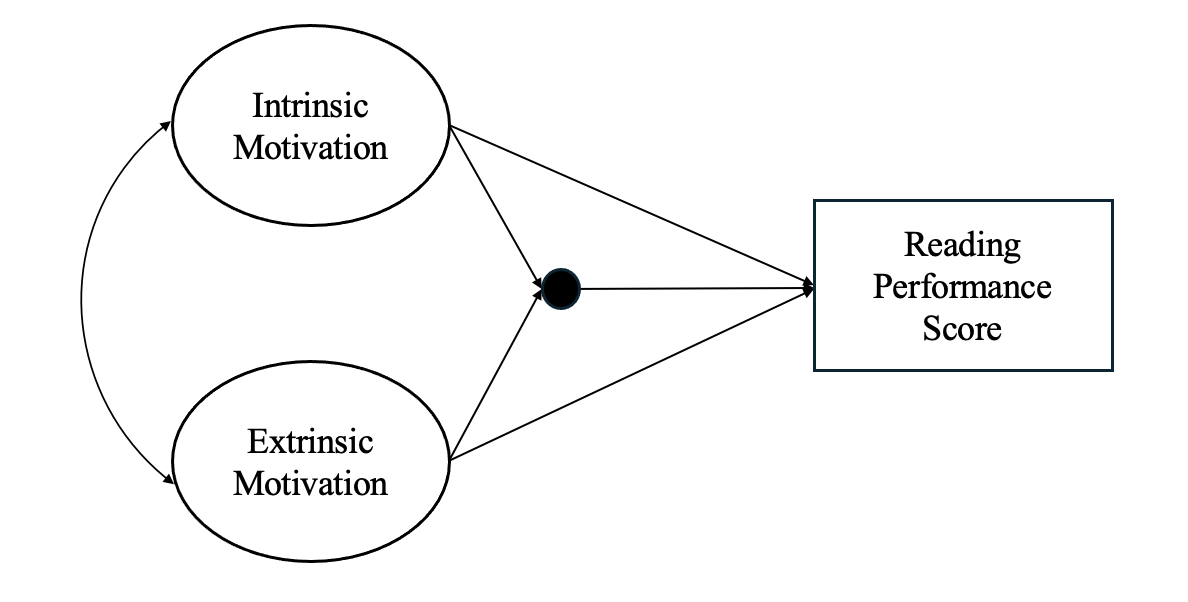
\includegraphics[width=0.8\textwidth]{/Users/jimmy_z/R Projects/2SPA-Int/Paper/Qual 1 Paper Draft/PIRL_Plot.png}
\caption{Structural Model of Illustrative Example from Park (2011).}
\caption*{\textit{Note. The model includes two first-order latent variables, intrinsic motivation and extrinsic motivation, depicted as ellipses. Their latent interaction term was depicted as a filled black circle. The dependent variable was observed and rendered as a rectangle.}}
\end{figure}

\section{Discussion}\label{discussion}

Applied researchers often explore complex relationships between variables, such as interactions. However, classical regression models, which assume that variables are free from measurement error, have been shown to yield biased estimates. As a result, latent variable approaches within the SEM framework are gaining prominence. In this study, we reviewed and compared the performance of three latent interaction methods, matched-pair UPI, RAPI, and 2S-PA-Int, in estimating interaction effects on congeneric items with varying factor loadings and measurement errors. Additionally, the regression-based approach using observed indicators, MMR, was included as a reference method.

We extended the 2S-PA model by Lai and Hsiao (2022) to support latent interaction estimation, naming it 2S-PA-Int. The primary distinction between matched-pair UPI, RAPI, and 2S-PA-Int lies in the formation of the latent interaction term. Matched-pair UPI constructs the latent interaction term using multiple product indicators (PIs) generated from first-order indicators, making it a multiple-indicator method. In contrast, RAPI and 2S-PA-Int use composite scores and factor scores as single indicators (SIs) for the latent interaction term, respectively.

Our results demonstrated that the MMR approach, based on observed indicators, consistently yielded substantially negative estimates of interaction effect path coefficients across multiple conditions. This finding can be attributed to the method's failure to properly account for measurement errors in the observed composites. These underestimated coefficients are consistent with previous research, which has emphasized the bias introduced by imperfect reliability when assessing interaction effects (Dunlap \& Kemery, 1988; Evans, 1985).

On the other hand, the latent interaction methods were capable of producing unbiased estimates of interaction effects by accounting for measurement errors, with the standardized bias (SB) and raw bias (RB) values consistently falling below the 0.40 threshold. However, RAPI and UPI exhibited notably positive SB values, indicating a tendency to overestimate interaction effects when true effects were present. These results are consistent with previous findings by Marsh et al. (2004) (using congeneric items with varying factor loadings), Hsiao et al. (2018) (using tau-equivalent items with varied error variances), and Hsiao et al. (2021) (using congeneric items), where matched-pair UPI and RAPI slightly overestimated interaction coefficients, albeit within acceptable limits. 2S-PA-Int also slightly tend to overestimate the path coefficient of interaction effects when they truly exist, indicating that latent interaction methods should be used with caution, particularly when researchers seek more conservative estimates of interaction effects.

With respect to coverage rates, RAPI demonstrated notably high coverage rates, ranging from 95\% to 97\% within the 95\% confidence interval (CI), indicating greater precision in capturing true interaction effects compared to matched-pair UPI and 2S-PA-Int. While slightly lower than those of RAPI, 2S-PA-Int also achieved acceptable coverage rates (93\% \textasciitilde{} 96\%), suggesting its capacity for accurately capturing true interaction effects. In contrast, matched-pair UPI was more susceptible to small sample sizes and low reliability levels, underscoring its reduced robustness in such conditions. These results imply that both RAPI and 2S-PA-Int possess sufficient capability of effectively detecting interaction effects across varied conditions. However, matched-pair UPI's performance was less consistent, particularly when error variances differed among first-order indicators. This observation is in line with previous studies, though it should be noted that Marsh et al.~(2004) did not evaluate matched-pair UPI with fully congeneric items, which may partly explain its reduced ability to capture true effects under such conditions.

MMR failed to show sufficient coverage rates across almost all conditions, indicating that this approach struggles to capture the true interaction effects within the specified confidence intervals. By ignoring measurement error, MMR produces narrower confidence intervals and underestimates the variability in the interaction effect, which results in increasing the likelihood of missing the true effects. Although latent interaction methods can correct for bias in SE estimation, Hsiao and Lai (2018) noted that constraining measurement errors for highly reliable variables may lead to over-adjustment, particularly in small sample sizes. Our RMSE results supported this concern, as latent interaction methods generally exhibited higher RMSE values compared to MMR when the sample size was 100. However, among the latent interaction methods, 2S-PA-Int produced the lowest RMSE values, which were nearly comparable to those of MMR. Overall, latent interaction methods for composite scores are preferable to MMR when considering both precision and bias in the estimation of interaction effect, with 2S-PA-Int demonstrating the greatest potential among the methods.

In our analysis of latent interaction methods, sample size and reliability level significantly influenced the estimation of non-zero interaction effects. Smaller sample sizes and higher measurement error, indicated by lower reliability, resulted in larger absolute values of SB and RB. However, as sample size increased and error decreased, both SB and RB improved across all methods, suggesting better performance with larger samples. Higher reliability levels also led to more unbiased estimates across conditions. Relative SE bias followed a similar trend, with smaller biases observed for larger sample sizes and higher reliability. As reported in the previous study (Hsiao \& Lai, 2018), RAPI generally exhibited greater relative SE bias than matched-pair UPI and 2S-PA-Int, especially under small sample sizes and low reliability, making it more prone to unstable interaction estimates. In terms of RMSE, both sample size and reliability had a clear effect, with larger sample sizes and higher reliability reducing RMSE values and improving accuracy. Among the methods, 2S-PA-Int consistently showed lower RMSE values and greater stability, particularly in challenging conditions with small sample sizes and low reliability, highlighting its robustness in estimating latent interaction effects.

Revisiting Marsh's criteria for an effective latent interaction model, 2S-PA-Int stands out for its simplicity as a single-indicator method and its efficient use of information through factor scores based on all first-order indicators. Models burdened with excessive indicators often face convergence issues due to complex covariance structures, potentially resulting in non-identifiable models (Bollen, 1989). Moreover, Byrne (2016) points out that too many indicators can introduce redundancy, unnecessarily complicating the model and increasing the risk of estimation problems. Therefore, 2S-PA-Int emerges as a better alternative to matched-pair UPI, especially in cases of small sample size and low reliability. Compared to RAPI, 2S-PA-Int also offers greater stability and accuracy in estimating interaction effects.

\section{Limitations and Future Directions}\label{limitations-and-future-directions}

Marsh et al.~(2004) demonstrated that all-pair UPI was not preferred due to its lack of substantial improvement in latent interaction estimation, despite having a slightly more complex model compared to matched-pair UPI. In our preliminary study, we investigated the performance of all-pair UPI on congeneric items, as Marsh et al.~(2004) only examined parallel items without varying factor loadings and error variances. We found that while SB of interaction estimates produced by all-pair UPI were negligible for parallel items, they were more remarkable for congeneric factor items (with varied factor loadings but consistent error variances) and fully congeneric items. A likely explanation for the increased standardized biases is that, although RB values were very small across all item types, the corresponding standard errors systematically decreased as sample size increased. These results suggest that all-pair UPI did not perform as well as matched-pair UPI, which is why it was not included in our main study (Results of the preliminary simulation study of all-pair UPI are available at: \href{https://github.com/Gengrui-Zhang/2S-PA-Int/blob/main/Qual_1_Supplemental_Material/Supplemental-Material.pdf}{Supplemental Material}).

As a limitation of our study, we did not evaluate or compare alternative methods using distribution analytic approaches, such as the latent moderated structural equation (LMS; Klein \& Moosbrugger, 2000) method, since the focus was on product indicator methods. Previous research has shown that LMS tends to produce unbiased estimates of latent interaction effects with acceptable statistical power when applied to congeneric items with normal distributions (Hsiao et al., 2021; Cham et al., 2012). In future investigations, we plan to incorporate widely used alternative methods for comparison with the 2S-PA-Int approach.

Previous studies on latent interaction effects have generally employed simple designs with two latent predictors and one interaction term, which may not fully capture the complexity of real-world scenarios involving multiple interaction terms. Furthermore, multilevel designs are increasingly common in educational, counseling, and organizational research (e.g., students nested in classrooms, patients nested in clinics, employees nested in companies). It would be valuable to explore the potential of 2S-PA-Int in handling more complex data structures, varying sample sizes, and reliability levels in these multilevel contexts.

Another limitation, as noted by Hsiao et al.~(2018), is that RAPI may be more accessible when researchers are working with secondary data, where only composite scores and their reliability indices (e.g., Cronbach's \(\alpha\)) are typically available. In cases where factor scores and their standard errors are not reported, it may not be possible to compute factor scores, thus limiting the applicability of 2S-PA-Int. Additionally, the congeneric items in our study were continuous with normal distributions. Since categorical data are often used in psychological research to capture qualitative aspects of human behavior, attitudes, and characteristics (Brown, 2015; Kline, 2016), 2S-PA-Int has yet to be evaluated with categorical items. However, given its ability to incorporate observation-specific standard error of measurement for each observation, we expect 2S-PA-Int to perform well in estimating latent interaction effects with categorical data in future studies.

\newpage

\section{References}\label{references}

\phantomsection\label{refs}
\begin{CSLReferences}{1}{0}
\bibitem[\citeproctext]{ref-alginaNoteEstimatingJoreskogYang2001}
Algina, J., \& Moulder, B. C. (2001). A note on estimating the {J{ö}reskog-Yang} model for latent variable interaction using {LISREL} 8.3. \emph{Structural Equation Modeling}, \emph{8}(1), 40--52. \url{https://doi.org/10.1207/S15328007SEM0801_3}

\bibitem[\citeproctext]{ref-andersonComparisonBiasMean1996}
Anderson, L. E., Stone-Romero, E. F., \& Tisak, J. (1996). A {Comparison} of bias and mean squared error in parameter estimates of interaction effects: {Moderated} multiple regression versus error-in-variables regression. \emph{Multivariate Behavioral Research}, \emph{31}(1), 69--94. \url{https://doi.org/10.1207/s15327906mbr3101_5}

\bibitem[\citeproctext]{ref-bollenStructuralEquationsLatent1989d}
Bollen, K. A. (1989). \emph{Structural equations with latent variables} (pp. xiv, 514). John Wiley \& Sons. \url{https://doi.org/10.1002/9781118619179}

\bibitem[\citeproctext]{ref-bollenLatentVariablesPsychology2002a}
Bollen, K. A. (2002). Latent variables in psychology and the social sciences. \emph{Annual Review of Psychology}, \emph{53}(1), 605--634. \url{https://doi.org/10.1146/annurev.psych.53.100901.135239}

\bibitem[\citeproctext]{ref-bollenTestingStructuralEquation1993}
Bollen, K. A., \& Long, J. S. (Eds.). (1993). \emph{Testing structural equation models} (p. 320). Sage Publications, Inc.

\bibitem[\citeproctext]{ref-brownConfirmatoryFactorAnalysis2015}
Brown, T. A. (2015). \emph{Confirmatory factor analysis for applied research, 2nd ed} (pp. xvii, 462). The Guilford Press.

\bibitem[\citeproctext]{ref-browneAlternativeWaysAssessing1992}
Browne, M. W., \& Cudeck, R. (1992). Alternative ways of assessing model fit. \emph{Sociological Methods \& Research}, \emph{21}(2), 230--258. \url{https://doi.org/10.1177/0049124192021002005}

\bibitem[\citeproctext]{ref-byrneStructuralEquationModeling2016}
Byrne, B. M. (2016). \emph{Structural equation modeling with {AMOS}: {Basic} concepts, applications, and programming} (3rd ed.). Routledge. \url{https://doi.org/10.4324/9781315757421}

\bibitem[\citeproctext]{ref-carrollMeasurementErrorNonlinear2006}
Carroll, R. J., Ruppert, D., Stefanski, L. A., \& Crainiceanu, C. M. (2006). \emph{Measurement error in nonlinear models: {A} modern perspective, second edition} (2nd ed.). {Chapman and Hall/CRC}. \url{https://doi.org/10.1201/9781420010138}

\bibitem[\citeproctext]{ref-cartePursuitModerationNine2003b}
Carte, T. A., \& Russell, C. J. (2003). In pursuit of moderation: {Nine} common errors and their solutions. \emph{MIS Quarterly}, \emph{27}(3), 479--501. \url{https://doi.org/10.2307/30036541}

\bibitem[\citeproctext]{ref-chamEstimatingLatentVariable2012a}
Cham, H., West, S. G., Ma, Y., \& Aiken, L. S. (2012). Estimating latent variable interactions with non-normal observed data: {A} comparison of four approaches. \emph{Multivariate Behav Res}, \emph{47}(6), 840--876. \url{https://doi.org/10.1080/00273171.2012.732901}

\bibitem[\citeproctext]{ref-chinPartialLeastSquares2003}
Chin, W. W., Marcolin, B. L., \& Newsted, P. R. (2003). A partial least squares latent variable modeling approach for measuring interaction effects: {Results} from a {Monte Carlo} simulation study and an electronic-mail emotion/adoption study. \emph{Information Systems Research}, \emph{14}(2), 189--217. \url{https://doi.org/10.1287/isre.14.2.189.16018}

\bibitem[\citeproctext]{ref-cohenAppliedMultipleRegression2003}
Cohen, J., Cohen, P., West, S. G., \& Aiken, L. S. (2003). \emph{Applied multiple regression/correlation analysis for the behavioral sciences, 3rd ed} (pp. xxviii, 703). Lawrence Erlbaum Associates Publishers.

\bibitem[\citeproctext]{ref-collinsComparisonInclusiveRestrictive2001}
Collins, L. M., Schafer, J. L., \& Kam, C. M. (2001). \href{https://www.ncbi.nlm.nih.gov/pubmed/11778676}{A comparison of inclusive and restrictive strategies in modern missing data procedures}. \emph{Psychol Methods}, \emph{6}(4), 330--351.

\bibitem[\citeproctext]{ref-cronbachCoefficientAlphaInternal1951}
Cronbach, L. J. (1951). Coefficient alpha and the internal structure of tests. \emph{Psychometrika}, \emph{16}(3), 297--334. \url{https://doi.org/10.1007/BF02310555}

\bibitem[\citeproctext]{ref-cunninghamModerationSportManagement2019a}
Cunningham, G. B., \& Ahn, N. Y. (2019). Moderation in sport management research: {Room} for growth. \emph{Measurement in Physical Education and Exercise Science}, \emph{23}(4), 301--313. \url{https://doi.org/10.1080/1091367X.2018.1472095}

\bibitem[\citeproctext]{ref-daszykowskiRobustStatisticsData2007}
Daszykowski, M., Kaczmarek, K., Vander Heyden, Y., \& Walczak, B. (2007). Robust statistics in data analysis --- {A} review. \emph{Chemometrics and Intelligent Laboratory Systems}, \emph{85}(2), 203--219. \url{https://doi.org/10.1016/j.chemolab.2006.06.016}

\bibitem[\citeproctext]{ref-dekkingModernIntroductionProbability2005a}
Dekking, F. M., Kraaikamp, C., Lopuhaä, H. P., \& Meester, L. E. (2005). \emph{A {Modern Introduction} to {Probability} and {Statistics}}. Springer. \url{https://doi.org/10.1007/1-84628-168-7}

\bibitem[\citeproctext]{ref-devliegerHypothesisTestingUsing2016}
Devlieger, I., Mayer, A., \& Rosseel, Y. (2016). Hypothesis testing using factor score regression. \emph{Educ Psychol Meas}, \emph{76}(5), 741--770. \url{https://doi.org/10.1177/0013164415607618}

\bibitem[\citeproctext]{ref-estabrookComparisonFactorScore2013}
Estabrook, R., \& Neale, M. (2013). A comparison of factor score estimation methods in the presence of missing data: {Reliability} and an application to nicotine dependence. \emph{Multivariate Behav Res}, \emph{48}(1), 1--27. \url{https://doi.org/10.1080/00273171.2012.730072}

\bibitem[\citeproctext]{ref-foldnesChoiceProductIndicators2014}
Foldnes, N., \& Hagtvet, K. A. (2014). The choice of product indicators in latent variable interaction models: {Post} hoc analyses. \emph{Psychological Methods}, \emph{19}(3), 444--457. \url{https://doi.org/10.1037/a0035728}

\bibitem[\citeproctext]{ref-hancockReliabilityAradoxAssessing2011}
Hancock, G. R., \& Mueller, R. O. (2011). The reliability aradox in assessing structural relations within covariance structure models. \emph{Educational and Psychological Measurement}, \emph{71}(2), 306--324. \url{https://doi.org/10.1177/0013164410384856}

\bibitem[\citeproctext]{ref-harwellStrategyUsingBias2019}
Harwell, M. (2019). A strategy for using bias and {RMSE} as outcomes in {Monte Carlo} studies in statistics. \emph{J. Mod. Appl. Stat. Methods}, \emph{17}(2), jmasm.eP2938. \url{https://doi.org/10.22237/jmasm/1551907966}

\bibitem[\citeproctext]{ref-hsiaoEvaluationTwoMethods2018a}
Hsiao, Y.-Y., Kwok, O.-M., \& Lai, M. H. C. (2018). Evaluation of two methods for modeling measurement errors when testing interaction effects with observed composite scores. \emph{Educ Psychol Meas}, \emph{78}(2), 181--202. \url{https://doi.org/10.1177/0013164416679877}

\bibitem[\citeproctext]{ref-hsiaoModelingMeasurementErrors2021}
Hsiao, Y.-Y., Kwok, O.-M., \& Lai, M. H. C. (2021). Modeling measurement errors of the exogenous composites from congeneric measures in interaction models. \emph{Struct Equ Modeling}, \emph{28}(2), 250--260. \url{https://doi.org/10.1080/10705511.2020.1782206}

\bibitem[\citeproctext]{ref-huCutoffCriteriaFit1999}
Hu, L., \& Bentler, P. M. (1999). Cutoff criteria for fit indexes in covariance structure analysis: {Conventional} criteria versus new alternatives. \emph{Structural Equation Modeling}, \emph{6}(1), 1--55. \url{https://doi.org/10.1080/10705519909540118}

\bibitem[\citeproctext]{ref-huberRobustStatistics2011}
Huber, P. J. (2011). Robust {Statistics}. In M. Lovric (Ed.), \emph{International {Encyclopedia} of {Statistical Science}} (pp. 1248--1251). Springer. \url{https://doi.org/10.1007/978-3-642-04898-2_594}

\bibitem[\citeproctext]{ref-jackmanEstimatingLatentVariable2011a}
Jackman, G.-A., Leite, W., \& Cochrane, D. (2011). Estimating latent variable interactions with the unconstrained approach: {A} comparison of methods to form product indicators for large, unequal numbers of items. \emph{Structural Equation Modeling}, \emph{18}, 274--288. \url{https://doi.org/10.1080/10705511.2011.557342}

\bibitem[\citeproctext]{ref-joreskogStatisticalAnalysisSets1971}
Jöreskog, K. G. (1971). Statistical analysis of sets of congeneric tests. \emph{Psychometrika}, \emph{36}(2), 109--133. \url{https://doi.org/10.1007/BF02291393}

\bibitem[\citeproctext]{ref-joreskogLISRELStructuralEquation1993}
Jöreskog, K. G., \& Sörbom, D. (1993). \emph{{LISREL} 8: {Structural} equation modeling with the {SIMPLIS} command language} (pp. xvi, 202). Lawrence Erlbaum Associates, Inc.

\bibitem[\citeproctext]{ref-Jreskog1996NonlinearSE}
Jöreskog, K. G., \& Yang, F. (1996). \emph{Nonlinear structural equation models: {The Kenny-Judd} model with {Interaction} effects}.

\bibitem[\citeproctext]{ref-kennyEstimatingNonlinearInteractive1984a}
Kenny, D. A., \& Judd, C. M. (1984). Estimating the nonlinear and interactive effects of latent variables. \emph{Psychological Bulletin}, \emph{96}(1), 201--210. \url{https://doi.org/10.1037/0033-2909.96.1.201}

\bibitem[\citeproctext]{ref-kleinMaximumLikelihoodEstimation2000a}
Klein, A., \& Moosbrugger, H. (2000). Maximum likelihood estimation of latent interaction effects with the {LMS} method. \emph{Psychometrika}, \emph{65}(4), 457--474. \url{https://doi.org/10.1007/BF02296338}

\bibitem[\citeproctext]{ref-klinePrinciplesPracticeStructural2016}
Kline, R. B. (2016). \emph{Principles and practice of structural equation modeling, 4th ed} (pp. xvii, 534). Guilford Press.

\bibitem[\citeproctext]{ref-kyriazosAppliedPsychometricsSample2018}
Kyriazos, T. (2018). Applied psychometrics: {Sample} size and sample power considerations in factor analysis ({EFA}, {CFA}) and {SEM} in general. \emph{Psychology}, \emph{09}, 2207--2230. \url{https://doi.org/10.4236/psych.2018.98126}

\bibitem[\citeproctext]{ref-laiTwostagePathAnalysis2022a}
Lai, M. H. C., \& Hsiao, Y.-Y. (2022). Two-stage path analysis with definition variables: {An} alternative framework to account for measurement error. \emph{Psychological Methods}, \emph{27}(4), 568--588. \url{https://doi.org/10.1037/met0000410}

\bibitem[\citeproctext]{ref-laiCorrectingUnreliabilityPartial2023}
Lai, M. H. C., Tse, W. W.-Y., Zhang, G., Li, Y., \& Hsiao, Y.-Y. (2023). Correcting for unreliability and partial invariance: {A} two-stage path analysis approach. \emph{Structural Equation Modeling: A Multidisciplinary Journal}, \emph{30}(2), 258--271. \url{https://doi.org/10.1080/10705511.2022.2125397}

\bibitem[\citeproctext]{ref-linStructuralEquationModels2010b}
Lin, G.-C., Wen, Z., Marsh, H. W., \& Lin, H.-S. (2010). Structural equation models of latent interactions: {Clarification} of orthogonalizing and double-mean-centering strategies. \emph{Structural Equation Modeling: A Multidisciplinary Journal}, \emph{17}(3), 374--391. \url{https://doi.org/10.1080/10705511.2010.488999}

\bibitem[\citeproctext]{ref-lordStatisticalTheoriesMental1968}
Lord, F. M., Novick, M. R., \& Birnbaum, A. (1968). \emph{Statistical theories of mental test scores}. Addison-Wesley.

\bibitem[\citeproctext]{ref-mackinnonHowWhomMediation2008a}
MacKinnon, D. P., \& Luecken, L. J. (2008). How and for whom? {Mediation} and moderation in health psychology. \emph{Health Psychol}, \emph{27}(2S), S99--S100. \url{https://doi.org/10.1037/0278-6133.27.2(Suppl.).S99}

\bibitem[\citeproctext]{ref-marshStructuralEquationModels2004a}
Marsh, H. W., Wen, Z., \& Hau, K.-T. (2004). Structural equation models of latent interactions: Evaluation of alternative estimation strategies and indicator construction. \emph{Psychol Methods}, \emph{9}(3), 275--300. \url{https://doi.org/10.1037/1082-989X.9.3.275}

\bibitem[\citeproctext]{ref-martinProgressInternationalReading2007}
Martin, M. O., Mullis, I. V. S., \& Kennedy, A. M. (2007). \emph{Progress in {International Reading Literacy Study} ({PIRLS}): {PIRLS} 2006 {Technical Report}}. International Association for the Evaluation of Educational Achievement.

\bibitem[\citeproctext]{ref-maslowskyEstimatingInterpretingLatent2015a}
Maslowsky, J., Jager, J., \& Hemken, D. (2015). Estimating and interpreting latent variable interactions: {A} tutorial for applying the latent moderated structural equations method. \emph{Int J Behav Dev}, \emph{39}(1), 87--96. \url{https://doi.org/10.1177/0165025414552301}

\bibitem[\citeproctext]{ref-mcdonaldTheoreticalFoundationsPrincipal1970}
McDonald, R. P. (1970). The theoretical foundations of principal factor analysis, canonical factor analysis, and alpha factor analysis. \emph{British Journal of Mathematical and Statistical Psychology}, \emph{23}(1), 1--21. \url{https://doi.org/10.1111/j.2044-8317.1970.tb00432.x}

\bibitem[\citeproctext]{ref-moulderComparisonMethodsEstimating2002a}
Moulder, B. C., \& Algina, J. (2002). Comparison of methods for estimating and testing latent variable interactions. \emph{Structural Equation Modeling}, \emph{9}(1), 1--19. \url{https://doi.org/10.1207/S15328007SEM0901_1}

\bibitem[\citeproctext]{ref-muellerStructuralEquationModeling1997a}
Mueller, R. O. (1997). Structural equation modeling: {Back} to basics. \emph{Structural Equation Modeling}, \emph{4}(4), 353--369. \url{https://doi.org/10.1080/10705519709540081}

\bibitem[\citeproctext]{ref-muthenHowUseMonte2002}
Muthén, L. K., \& Muthén, B. O. (2002). How to use a {Monte Carlo} study to decide on sample size and determine power. \emph{Structural Equation Modeling: A Multidisciplinary Journal}, \emph{9}(4), 599--620. \url{https://doi.org/10.1207/S15328007SEM0904_8}

\bibitem[\citeproctext]{ref-radloffCESDScaleSelfreport1977b}
Radloff, L. S. (1977). The {CES-D} scale: {A} self-report depression scale for research in the general population. \emph{Applied Psychological Measurement}, \emph{1}(3), 385--401. \url{https://doi.org/10.1177/014662167700100306}

\bibitem[\citeproctext]{ref-raykovEstimationCompositeReliability1997}
Raykov, T. (1997). Estimation of composite reliability for congeneric measures. \emph{Applied Psychological Measurement}, \emph{21}(2), 173--184. \url{https://doi.org/10.1177/01466216970212006}

\bibitem[\citeproctext]{ref-rousseeuwAlternativesMedianAbsolute1993}
Rousseeuw, P. J., \& Croux, C. (1993). Alternatives to the {Median Absolute Deviation}. \emph{Journal of the American Statistical Association}, \emph{88}(424), 1273--1283. \url{https://doi.org/10.2307/2291267}

\bibitem[\citeproctext]{ref-rousseeuwRobustStatisticsOutlier2011}
Rousseeuw, P. J., \& Hubert, M. (2011). Robust statistics for outlier detection. \emph{WIREs Data Mining and Knowledge Discovery}, \emph{1}(1), 73--79. \url{https://doi.org/10.1002/widm.2}

\bibitem[\citeproctext]{ref-schoemannTestingInterpretingLatent2021}
Schoemann, A. M., \& Jorgensen, T. D. (2021). Testing and interpreting latent variable interactions using the {semTools} package. \emph{Psych}, \emph{3}(3), 322--335. \url{https://doi.org/10.3390/psych3030024}

\bibitem[\citeproctext]{ref-steinmetzThreeApproachesEstimate2011a}
Steinmetz, H., Davidov, E., \& Schmidt, P. (2011). Three approaches to estimate latent interaction effects: {Intention} and perceived behavioral control in the theory of planned behavior. \emph{Methodological Innovations Online}, \emph{6}(1), 95--110. \url{https://doi.org/10.4256/mio.2010.0030}

\bibitem[\citeproctext]{ref-tenbergeGreatestLowerBound2004}
Ten Berge, J. M. F., \& Sočan, G. (2004). The greatest lower bound to the reliability of a test and the hypothesis of unidimensionality. \emph{Psychometrika}, \emph{69}(4), 613--625. \url{https://doi.org/10.1007/BF02289858}

\bibitem[\citeproctext]{ref-wuComparisonStrategiesForming2013}
Wu, Y., Wen, Z., Marsh, H., \& Hau, K.-T. (2013). A comparison of strategies for forming product indicators for unequal numbers of items in structural equation models of latent interactions. \emph{Structural Equation Modeling: A Multidisciplinary Journal}, \emph{20}, 551--567. \url{https://doi.org/10.1080/10705511.2013.824772}

\end{CSLReferences}


\end{document}
